\documentclass[pre,aps,floatfix,10pt,superscriptaddress, notitlepage,preprint]{revtex4-1}
\pdfoutput=1
\usepackage[english]{babel}
\usepackage[T1]{fontenc}
\usepackage[latin9]{inputenc}
\usepackage{amsmath,amssymb}
\usepackage[svgnames]{xcolor}
\usepackage{graphicx}
\usepackage{acro}
\usepackage{subfig}
\usepackage{caption}
\graphicspath{{figures/}}

\captionsetup[figure]{justification=raggedright}

\newcommand{\set}[1]{\ensuremath{\mathcal{#1}}}

\DeclareAcronym{pdf}{
  short=PDF,
  long=Probability Density Function,
}
\DeclareAcronym{iid}{
  short=i.i.d.,
  long=Independent Identically Distributed
}
\DeclareAcronym{ou}{
  short=OU,
  long=Ornstein-Uhlenbeck,
}
\DeclareAcronym{gktl}{
  short=GKTL,
  long=Giardina-Kurchan-Tailleur-Lecomte,
}
\DeclareAcronym{ams}{
  short=AMS,
  long=Adaptive Multilevel Splitting,
}
\DeclareAcronym{tams}{
  short=TAMS,
  long=Trajectory Adaptive Multilevel Splitting,
}
\DeclareAcronym{scgf}{
  short=SCGF,
  long=Scaled Cumulant Generating Function,
}
\DeclareAcronym{lbm}{
  short=LBM,
  long=Lattice Boltzmann Method,
}
\DeclareAcronym{lbe}{
  short=LBE,
  long=Lattice Boltzmann Equation,
}
\DeclareAcronym{lgca}{
  short=LGCA,
  long=Lattice Gas Cellular Automata,
}
\DeclareAcronym{lbgk}{
  short=LBGK,
  long=Lattice Bhatnagar-Gross-Krook
}
\DeclareAcronym{OU}{
  short=OU,
  long=Ornstein--Ulhenbeck
}
\DeclareAcronym{dns}{
  short=DNS,
  long=Direct Numerical Simulation,
}
\DeclareAcronym{md}{
  short=MD,
  long=Molecular Dynamics,
}
\DeclareAcronym{cfd}{
  short=CFD,
  long=Computational Fluid Dynamics,
}

\begin{document}
	
\title{Importance sampling applied to the simulation of extreme mechanical efforts exerted by a turbulent flow on a bluff body}

\author{Thibault Lestang}
\email{thibault.lestang@ens-lyon.fr}
\affiliation{Univ Lyon, ENS de Lyon, Univ Claude Bernard de Lyon, CNRS, Laboratoire de Physique, F-69342 Lyon, France}
\affiliation{Univ Lyon, Ecole Centrale de Lyon, Univ Claude Bernard de Lyon, Insa de Lyon, CNRS, Laboratoire de M\'ecanique des Fluides et d'Acoustique, F-69134 Ecully cedex, France}
\author{Freddy Bouchet}
\email{freddy.bouchet@ens-lyon.fr}
\affiliation{Univ Lyon, ENS de Lyon, Univ Claude Bernard de Lyon, CNRS, Laboratoire de Physique, F-69342 Lyon, France}
\author{Emmanuel L�v�que}
\email{emmanuel.leveque@ec-lyon.fr}
\affiliation{Univ Lyon, Ecole Centrale de Lyon, Univ Claude Bernard de Lyon, Insa de Lyon, CNRS, Laboratoire de M\'ecanique des Fluides et d'Acoustique, F-69134 Ecully cedex, France}



\begin{abstract}
This study evaluates the relevance of importance sampling techniques to optimize the numerical simulation of extreme mechanical efforts exerted by a turbulent flow impinging onto a bluff body. The main idea behind importance sampling is here to replace a long simulation by a set of shorter simulations running in parallel with dynamics that are replicated or abandoned in order to sample large events more frequently. 
%
Such techniques have already proved their efficiency for simulating extreme events in... with significant run-time savings.
Application to turbulent fluid-mechanical systems remains mainly open. 
%
The drag experienced by a squared obstacle placed in a turbulent flow (in two dimensions) is taken as a representative case study to investigate the performance of two important sampling algorithms, namely .... 
Practical evidence is given that these algorithms allow for the correct sampling of rare large-amplitude drag events and the estimation of return times with a reduced computational effort... However, limitations... pitfalls... 
Importantly, such techniques also provide access to the flow scenario yielding extreme events. In the present case, it is found that... blocking effect
\end{abstract}

\maketitle

\section{Introduction}

// Recall the previous success of importance sampling techniques with references. //
Explain why interesting to test application for turbulent systems. // To what extent a turbulent system is different from previous case studies? // 
\\

Turbulent flows are important in a variety of natural phenomena, industrial and civil applications with the characteristic feature to spontaneously develop intense and sporadic fluid motions associated with enormous internal forces. In the turbulence literature, ``extreme'' can refer to fluctuations that deviate from the mean value by $O(10)$ standard deviations. // true ? //
The nature of such extreme dynamical events and their statistics are of crucial interest to predict excessive mechanical efforts that may cause damages and threaten the structural integrity of embedded structures.
\\

From the viewpoint of dynamical systems, turbulence in fluids has to do with non-linearity and strong departure from statistical equilibrium. The use of perturbative methods in identifying resonant interactions (among degrees of freedom)  leading to extreme fluctuations is not successful. 
In this context, simulation offers a practical means to gain insight into the extreme events. However, their numerical sampling requires long simulation since these events are rare as well. 
\\


// Our motivations and expectations. // 


\section{Description of the case study}
\label{sec:test_flow}

\begin{figure}
  \centering
  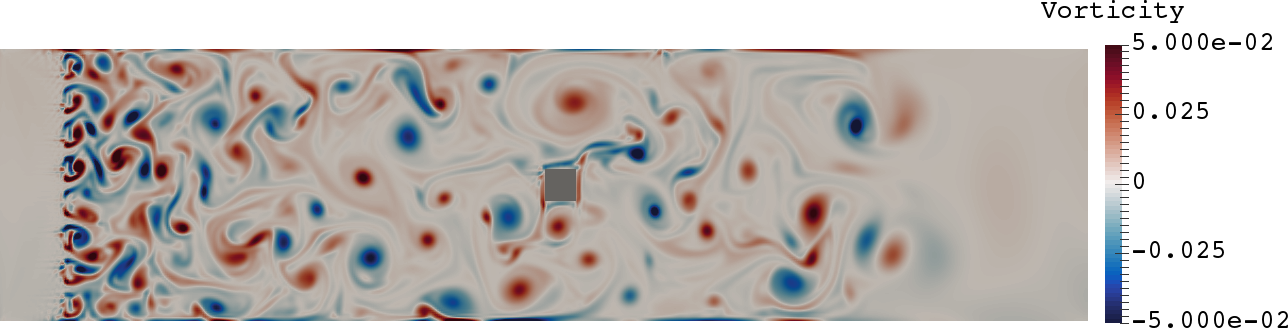
\includegraphics[width=\linewidth]{illustr_vort/illustration_vorticity_tf2.png}
  \caption{Our case study is a grid-generated turbulent flow impinging a squared obstacle located at the center of a channel (in two dimensions).  The vorticity is displayed with an arbitrary colormap from blue (negative values) to red (positive values). The Reynolds number based on the grid spacing is $Re=...$.  // no color bar, show the grid //}
  \label{fig:computational_domain}
\end{figure}

The drag exerted by a grid-generated turbulent flow onto a squared obstacle is considered as our representative case study. The flow is contained in a long channel as illustrated in Fig.~\ref{fig:computational_domain}. Although real-world applications would eventually imply three-dimensional dynamics, a simplified two-dimensional setting has been chosen here to reduce the computational cost and make possible a systematic study. 
Nevertheless, this fluid-mechanical system exhibits the characteristic features of turbulent fluid-structure interaction. // true even if 2d? // In the present situation, the obstacle does not deform or move. Through  this specific setting, our main motivation is to evaluate the operability of importance sampling techniques to capture extreme events with a significant run-time savings.  
\\

A constant parabolic profile is imposed for the streamwise velocity at the inlet of the channel and turbulence is generated by means of a grid. 
At the outlet of the channel, the flow is progressively damped within a \textit{sponge layer}~\cite{ref1,ref2} where the viscosity is artificially enhanced. 
% Such sponge layer facilitates the implementation of an open boundary at the outlet, where a zero momentum flux along the mean-flow direction in imposed.
\\

Turbulent eddies are generated in the near-wake of the grid and carried downstream. // grid is usually characterized by the spacing and the mesh size, are they equal here? //
They interact with each other and grow in size as expected in two-dimensional turbulence. 
The size of the eddies that eventually hit the square (at the center of the channel) is comparable to the size of this obstacle, which results in strong fluctuations of the drag acting on the square. 
\\


The flow dynamics are computed by the lattice Boltzmann (LB) method ~\cite{ref1,ref2}. 
While standard numerical methods rely on the discretization of the Navier-Stokes equations, the LB method emerged in the late 80s as a conceptually different approach. Fluid motions are simulated at a mesoscopic level that is intermediate between the microscopic and the macroscopic. Capturing the kinetic behavior of collections of fluid particles distributed on a lattice is here preferred to solving non-linear PDEs. This seems crazy, however, most details at the mesoscopic level play actually no role at the macroscopic level. Therefore, kinetic equations simpler than the original Boltzmann equation may be designed by retaining only the basic features that pertain at the macroscopic level. This is, in short, the rationale behind the LB approach. In our situation, the LB method has been chosen principally for its outstanding computational efficiency.  
%
More precisely, the fluid is viewed as populations of particles
that collide, redistribute and propagate along the different links of a discrete lattice. 
In our two-dimensional situation, the so-called D2Q9 lattice with only nine possible velocities $\{\mathbf{c_i}\}_{i=0...8}$ at each node has been adopted (see Fig.~\ref{fig:D2Q9}).
Locally, the macroscopic flow variables (per unit volume) are recovered by summing over the densities of particles $\{f_i\}_{i=0...8}$ moving with the different velocities, i.e.
\[
\rho(\mathbf{x},t) = \sum_i f_i(\mathbf{x},t) \quad \mathrm{and}\quad \rho(\mathbf{x},t) \mathbf u(\mathbf{x},t) = \sum_i f_i(\mathbf{x},t) \mathbf{c_i}
\]
for the mass density and the fluid momentum respectively. The assumption of weak compressibility (for an ideal gas) is made so that the pressure is directly proportional to the mass density: $p = c_s^2 \rho$ where $c_s$ is interpreted as a speed of sound.  

\begin{figure}
	\centering
	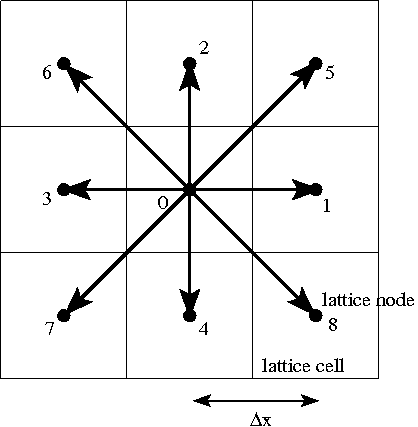
\includegraphics[width=0.3\linewidth]{D2Q9/D2Q9}
	\caption{Sketch of the D2Q9 lattice. Particles move exactly from a lattice node towards one of its nine neighbours (including the node itself) during one time step. By definition, the lattice spacing is related to the time step by $\Delta x/ \Delta t = \sqrt{3} c_s$, where $c_s$ is interpreted as a speed of sound.}
	\label{fig:D2Q9}
\end{figure}


The complexity of the flow emerges from the repeated application of simple rules of streaming and collision. Therefore, the LB scheme advances the local densities of particles $f_i(\mathbf{x},t)$ moving with velocities $\mathbf{c}_i$  in a two-step procedure. Namely, an \emph{exact} streaming step 
\[
f_i(\mathbf{x}+\mathbf{c}_i \Delta t, t + \Delta t) = f_i^{\mathrm{out}}(\mathbf{x},t)
\]
during which particles move with their own velocity to a neighboring node, is consecutive to an instantaneous collision step
\[
f_i^{\mathrm{out}}(\mathbf{x},t) = -\frac 1 {\tau_\nu} \left(f_i(\mathbf{x},t) - f_i^\mathrm{eq}(\mathbf{x},t) \right)
\]
which can be viewed as the relaxation of local densities towards an absolute equilibrium at the macroscopic level; the time-scale $\tau_\nu$ is related to the kinematic viscosity of the fluid by 
\[
\nu = \left( {\tau_\nu} - \frac 1 2 \right) c_s^2 ~\Delta t
\]
This simplification of the collision kernel is known as the BGK approximation in the kinetic theory of gas. The equilibrium function is given (assuming Einstein summation convention) by
\[
f_i^\mathrm{eq}(\mathbf{x},t) = w_i  \rho(\mathbf{x},t) \left( 1 + \frac{\mathrm u(\mathbf{x},t) \cdot \mathbf{c_i}}{c_s^2} +
\frac{u_\alpha(\mathbf{x},t) u_\beta(\mathbf{x},t)({c_i}_\alpha {c_i}_\beta - c_s^2 \delta_{\alpha\beta})}{2 c_s^4} \right)
\] 
with the weight factors $w_0=4/9,~w_{1...4} = 1/9$ and $w_{5...8}=1/36$ for the D2Q9 lattice. 
Finally, let us mention that this discrete LB scheme is second-order accurate in $\Delta x $ and compliant to the weakly-compressible Navier-Stokes equations (with a third-order error in $\mathrm{Ma}=|\mathbf{u}|/c_s$) as the lattice spacing vanishes, i.e. $\Delta x \to 0$. 


// algorithm for boundary conditions // computation of the stress with LBM // grid resolution, number of grid points in each direction, Reynolds, Mach numbers, etc. // low Mach number approaches the nearly-incompressible limit
\\

As mentioned before, the pressure is directly accessible from the mass density: $p = \rho c_s^2$. The viscous stress is also obtained easily from the densities of particles by
\[
\tau^\mathrm{visc.}_{\alpha \beta} = -\frac{\nu}{\tau_\nu ~ c_s^2 \Delta t} \sum_i  {c_i}_\alpha {c_i}_\beta (f_i - f_i^\mathrm{eq})
\]
so that the total stress expresses as
\begin{equation}\label{eq:def_stress}
\tau_{\alpha \beta} = -  c_s^2 \sum_i f_i ~ \delta_{\alpha\beta}  - \frac{\nu}{\tau_\nu ~ c_s^2 \Delta t} \sum_i  {c_i}_\alpha {c_i}_\beta (f_i - f_i^\mathrm{eq})
\end{equation}

\subsection{The drag force}
\label{sec:drag_force}

The incoming turbulent flow exerts fluctuating mechanical efforts onto the squared obstacle. The \textit{drag} is defined as the resulting force in the streamwise $x$-direction and reads 
\begin{equation}
  \label{eq:drag_definition}
  f_d(t) = \int_{\mathcal{S}} \boldsymbol{\tau}_{x \beta}(\mathbf{x},t) ~ \mathrm{d}{\mathcal{S}}_\beta(\mathbf{x})  
\end{equation}
where $\mathcal{S}$ is the surface of the obstacle. 
In our situation, the viscous stress makes a negligible contribution to the drag. This latter therefore results mostly from pressure forces, which are closely related to the distribution of velocity gradients in the vicinity of the obstacle (in the nearly-incompressible limit). 
%
Since the pressure on the top and bottom sides of the square applies in the normal direction, they do not contribute to the drag. 
As a consequence, the drag may be viewed as the pressure difference 
\begin{equation}
  \label{eq:drag_approx}
  f_d(t) = p_{fb}(t) - p_{b}(t)
\end{equation}
where $p_{fb}(t)$ and $p_{b}(t)$ denote the pressure integrated over the forebody and the base of the obstacle, respectively.

%% The phenomenology of typical drag fluctuations
The typical timescale of variation of the drag therefore corresponds to the timescale of pressure fluctuations in the vicinity of the obstacle.
An estimate of such timescale is the \textit{turnover time}
\begin{equation}
  \label{eq:turnover_time}
  \tau_0 = \frac{R}{U},
\end{equation}
where $R$ is the diameter of the cylinder and $U$ the mean-flow velocity.
Figure~\ref{fig:typical_drag_signal} illustrates the time evolution of the drag acting on the square obstacle over a few thousands turnover times.
The evolution over a few turnover times of the vorticity field around the obstacle is displayed in figure~\ref{fig:typical_vorticity}.
One can see that the interaction of the incoming flow with the square obstacle primarily results in boundary layers along the top and bottom boundaries.
However, the vorticity corresponding to these boundary layers only have a small impact on the the pressure field in the vicinity of the obstacle, because it is rapidly advected dowmstream by the mean-flow.
As a consequence, the base pressure varies much less than the forebody pressure, and typical drag fluctuations mostly result from the fluctuating pressure at the front of the obstacle.

In the following section~\ref{sec:direct_sampling}, we highlight a very different phenomenology for \textit{extreme} fluctuations of the drag acting on the obstacle.
In particular, we show that extreme fluctuations mainly result from fluctuations of the base pressure, whereas forebody pressure fluctuations play a smaller role.

\begin{figure}
  \centering
  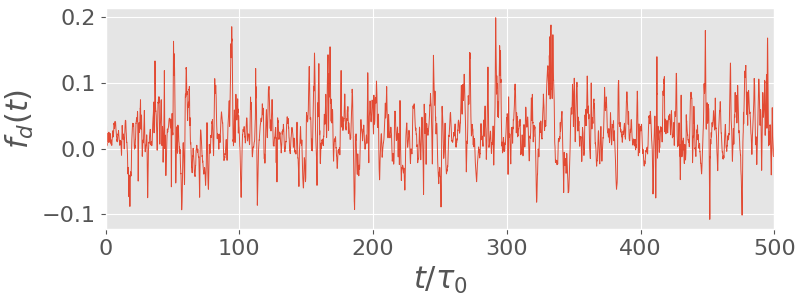
\includegraphics[width=0.7\linewidth]{typical_drag_signal/typical_drag_signal.png}
  \caption{Typical temporal evolution of the drag acting on the square cylinder pictured in figure~\ref{fig:computational_domain}. The correlation time $\tau_c$ is defined further in this text and correspond to the typical fluctuation timescale of the drag.}
  \label{fig:typical_drag_signal}
\end{figure}
\begin{figure}
  \centering
  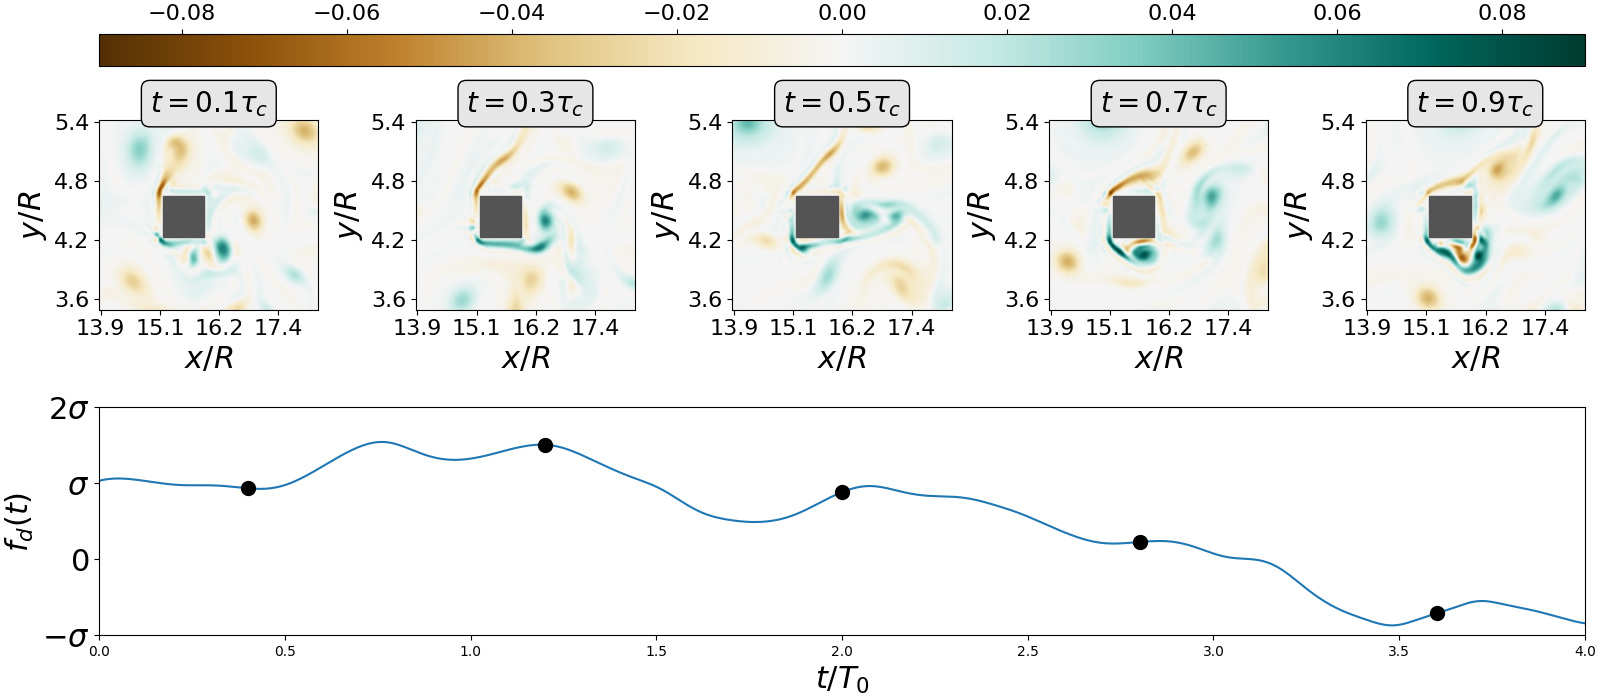
\includegraphics[width=\linewidth]{ecoulement_typique/ecoulement_typique.png}
  \caption{Vorticity dynamics corresponding to typical drag fluctuations over one correlation time unit $\tau_c$. Negative vorticity is generated along the bottom boundary, and advected away from the the obstacle by the mean flow.}
  \label{fig:typical_drag_signal}
\end{figure}

\subsection{The drag random process: Probability Density Function, time correlations}
\label{sec:pdfs}

\begin{figure}
  \centering
    \subfloat[]{\label{fig:pdf_drag_a}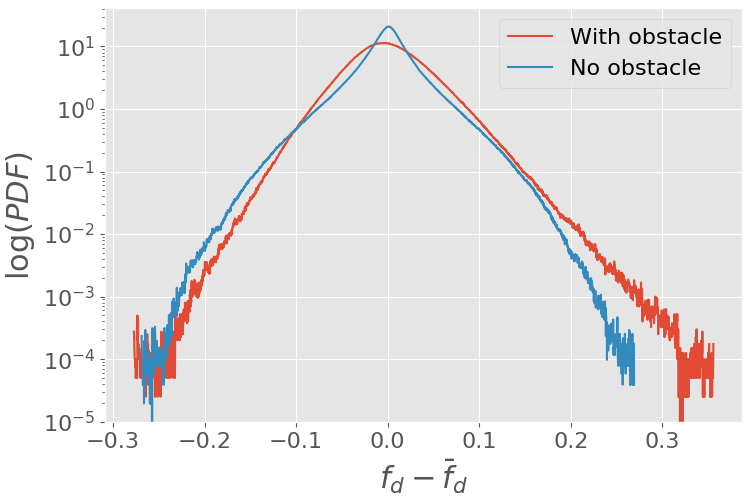
\includegraphics[width=.5\linewidth]{./PDF_drag/PDF_drag.png}}
    \subfloat[]{\label{fig:pdf_drag_b}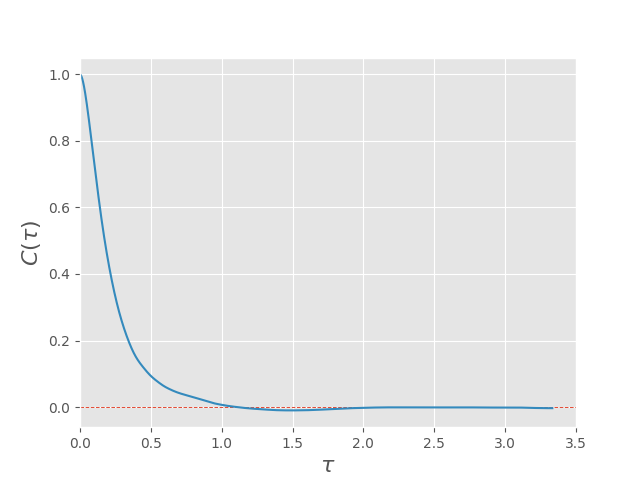
\includegraphics[width=.5\linewidth]{autocorr_drag/autocorr_drag.png}}  
  \caption{\textbf{(a)} \ac{pdf} describing the statistics of the instantaneous drag fluctuations, computed on the basis of the control timeseries. \textbf{(b)} Autocorrelation function for the instantaneous drag $f_d$, defined as $(\mathbb{E}[f_d(t+\tau)f_d(t)]-\mathbb{E}[f_d]^2)/\sigma^2$, computed over the control run. It shows the exponential decay of the correlations over time.}
  \label{fig:pdf_drag}
\end{figure}

In the following we consider the drag force acting on the obstacle as a scalar random process $f_d(t)$.
In order to estimate its statistical properties, we performed a simulation of the dynamics over a duration $T_{tot} = 4\times 10^6\tau_0$.
In the following of this paper we refer to this long simulation as the \textit{control run}.
Furthermore, we denote by $\bar{f}_d$ and $\sigma$ the average and variance computed over the control run, respectively.
Figure~\ref{fig:pdf_drag} displays an estimate of the \ac{pdf} for the drag process, computed on the basis of the control timeseries $\{f_d(t)\}_{0\leq t \leq T_{tot}}$ obtained from the control run.
One can see that the tails of this distribution, that describe the probability of very rare events, can be very well modelled by an exponential \ac{pdf} of the form $p(f_d) = \lambda^{-1}e^{-\lambda f_d}$.
In addition, figure~\ref{fig:pdf_drag} displays an estimate of the \ac{pdf} of the process describing the drag acting on a control surface equivalent to the surface of  the obstacle, in a flow \textit{without obstacle}.
This different setup is illustrated in figure~\ref{fig:no_square}.
In this case, the corresponding \ac{pdf} estimate for the drag process is quasi-symmetric and, more importantly, does not display exponential tails.
We conclude that the interation of the flow with the square obstacle is responsible for the exponential tails of the \ac{pdf} of the drag process.
In section~\ref{sec:time_avg}, we relate this very particular shape of the \ac{pdf} describing extreme drag fluctuations to the phenomenology of extreme fluctuations of the time-average of the drag process. 

Lastly, figure~\ref{fig:correlation_function} illustrates that the drag process has exponentially decaying time correlations.
In the following we call \textit{correlation time}, denoted by $\tau_c$, the typical time it takes for the drag process to decorrelate.
We observe that $\tau_c \approx \tau_0$.
This means that the drag decorrelates after only a few number of eddies interacted with the square obstacle.

% \begin{equation}
%   \label{eq:correlation_def}
%   C(\tau) = \frac{\mathbb{E}[f_d(t)f_d(t+\tau)] - \mathbb{E}^2[f_d]}{\sigma ^2} \quad \mbox{with} \quad \sigma^2 = \mathbb{f_d^2} - \mathbb{f_d}^2.
% \end{equation}

% As a consequence, temporal correlations in the drag process have a finite life time $\tau_c$---the \textit{correlation time}.

% From the point of view of the drag process, the system lost its memory after only a few eddies interacted with the obstacle.
% This observation has important consequences for the application of rare event algorithms, as will be discussed in section~\ref{sec:rare_events_algorithms}.

\section{Direct sampling of extreme fluctuations of the drag acting on a square cylinder in two-dimensional turbulence}
\label{sec:direct_sampling}

We now turn to a description of the phenomenology of extreme fluctuations of the drag that acts on the square cylinder mounted in the flow described in section~\ref{sec:test_flow}.

How rare is a fluctuation $f_d \geq a$ can be determined by computing its \textit{return time} $r(a)$.
It is defined as the average time between two consecutive occurrences of a fluctuation $f_d \geq a$.
Extreme drag fluctuations are \textit{rare events}, that is fluctuations for which $r(a) \gg \tau_c$.
In this context, the occurrence of the fluctuations follows a Poisson process and~\cite{lestang2018}
\begin{equation}
  \label{eq:return_time}
  r(a) \underset{a\to\infty}{\propto} \frac{1}{\mathbb{P}(f_d\geq a)} \propto e^{\alpha a}
\end{equation}
where $\alpha$ is the rate describing the positive tail of the drag \ac{pdf}, see figure~\ref{fig:pdf_drag}.
Figure~\ref{fig:return_time_instant} illustrates the fluctuation amplitude $a$ as a function of the return time $r(a)$, for the drag process $f_d(t)$.
Such plot can be obtained from a sample timeseries following a simple procedure~\cite{lestang2018}.

In the following we discuss extreme fluctuations of both the instantaneous drag $f_d$ and time-averaged drag with return times larger than $10^4\tau_c$.
In this section extreme drag fluctuations are simply sampled by simulating the flow over a very long duration.
This approach is referred to as \textit{direct sampling}, as opposed to approaches involving the use of rare events algorithms, discussed in section~\ref{sec:rare_events_algorithms}.
Such approach is made possible by the relative simplicity of the flow described in section~\ref{sec:test_flow}.
The control run mentioned in the previous section, spanning $T_{tot} = 10^6 \tau_c$, could be achieved in a wall-clock time of a few weeks and gives access to extreme fluctuations $f_d \geq a$ with a return time $r(a) \leq 10^6\tau_c$.
\subsection{Extracting extreme drag fluctuations from a very long timeseries}
\label{sec:extreme_extraction}

On the basis of the control timeseries $\{f_d(t)\}_{0 \leq t \leq T_{tot}}$, we tracked every drag fluctuation with an amplitude greater than a fixed threshold amplitude $a$.
The value of this threshold was chosen so that the return time of fluctuations with an amplitude larger than $a$ is $T_{tot}/100$.
Figure~\ref{return_time_instant} displays the fluctuation amplitude $a$ as a function of the return time.
According to Figure~\ref{return_time_instant}, the threshold amplitude $a$ is set to $7.6\sigma$ with $\sigma$ the standard deviation of the drag process.
We denote by $(t^{\star}, f_d^{\star})$ a fluctuation of peak amplitude $f_d^{\star}$ occurring at time $t^{\star}$, as illustrated in figure~\ref{fig:extraction}.
From the control timeseries, we identified $104$ independent extreme drag fluctuations whith an amplitude greater than $7.6\sigma$, \textit{i.e.} with a return time greater than $10^4\tau_c$.
In the following sections~\ref{sec:forebody_and_base_contribution} and~\ref{sec:instantaneous_drag}, we describe the phenomenology of extreme drag fluctuations on the basis of this set of
events.

\begin{figure}
  \centering
  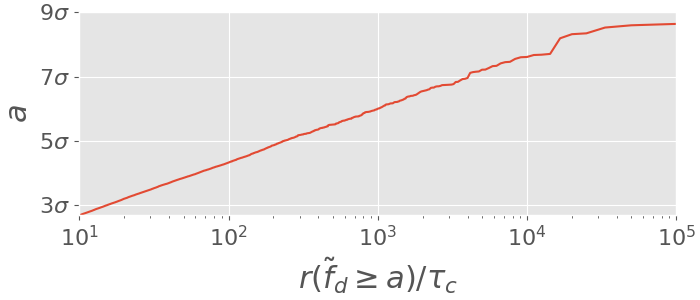
\includegraphics[width=.6\linewidth]{return_time/return_time.png}
  \caption{Drag fluctuation amplitude as a function the corresponding return time. Here $f_d$ denotes the centered and reduced drag with $f_d=0$ and $\sigma = 1$.}
  \label{fig:return_time_instant}
\end{figure}
\subsection{Instantaneous drag}
\label{sec:instantaneous_drag}

\subsubsection{Contribution of forebody and base pressure fluctuations to the overall drag fluctuation}
\label{sec:forebody_and_base_contribution}
In section~\ref{sec:test_flow}, we pointed out that typical drag fluctuations mainly originate from fluctuations of the forebody pressure, \textit{i.e.} pressure fluctuations resulting from the upstream turbulent flow.
We now investigate the relative contribution of forebody and base pressure fluctuations to the overall drag fluctuations, in the case of the sampled \textit{extreme} drag fluctuations.
Let $(t^{\star}, f_d^{\star})$ be an extreme drag event.
In the following we consider the effective fluctuation $\tilde{f}_d^{\star} = f_d^{\star} - \langle f_d \rangle$.
It can be further decomposed into 
\begin{equation}
  \tilde{f}_d^{\star} = \tilde{p}_{fb}^{\star} - \tilde{p}_{base}^{\star},
\end{equation}
where $\tilde{p}_{fb}^{\star}$ and $\tilde{p}_{base}^{\star}$ denote the fluctuation of the forebody pressure and base pressure, respectively, that is $\tilde{p}_{base}^{\star} = p_{base}^{\star} - \langle p_{base} \rangle$ .
Figure~\ref{fig:contribution_forebody_and_base_pressure} shows the relative contributions $\tilde{p}_{base}^{\star}/\tilde{f}_d^{\star}$ and $\tilde{p}_{fb}^{\star}/\tilde{f}_d^{\star}$ to the overall drag fluctuation for the base and forebody pressure fluctuations, respectively.  
\begin{figure}
  \centering
  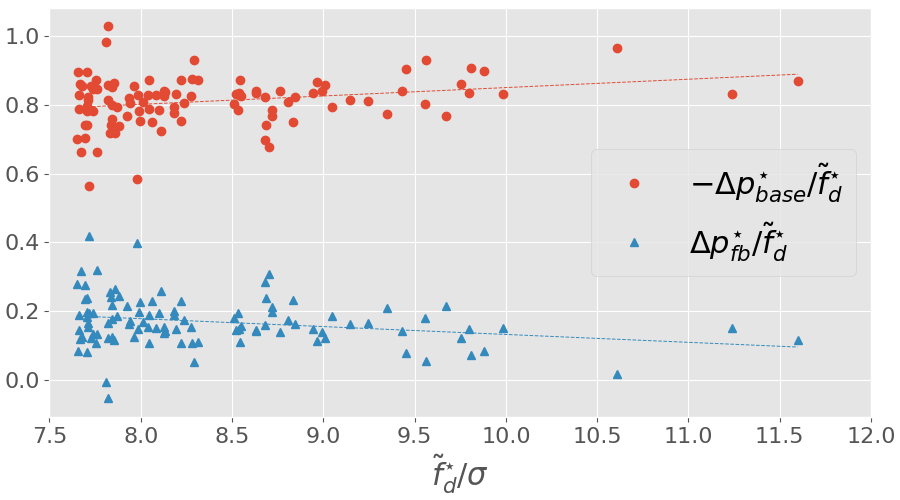
\includegraphics{pressure_ratio/pressure_ratio.png}
  \label{fig:pressure_ratio}
\end{figure}
It shows that among the 104 sampled extreme events, the base pressure fluctuation typically contributes for $80\%$ of the overall drag fluctuation.
By contrast with typical drag fluctuations, extreme fluctuations of the drag acting on the square cylinder are dominated by the variation of the pressure in the vicinity of the base of the obstacle.
In addition, figure~\ref{fig:pressure_ratio} hints that, the larger the fluctuation, the more important is the contribution of the base pressure fluctuation, relatively to the forebody pressure fluctuation.

\subsubsection{Dynamical aspects of extreme drag fluctuations}
\label{sec:dynamical_aspects}

\begin{figure}
  \centering
  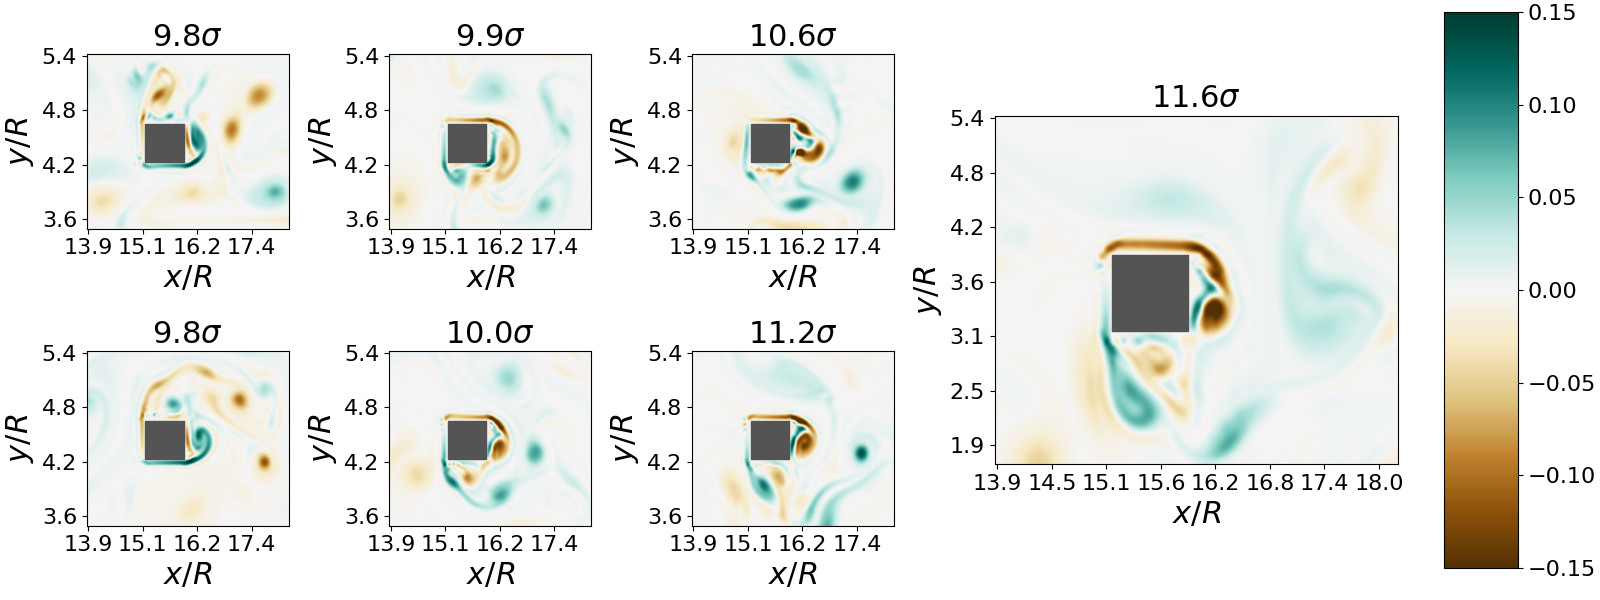
\includegraphics[width=.8\linewidth]{illustr_extrms_vorticity/illustr_extrms_vorticity.png}
  \caption{\label{fig:top_4_events_vorticity} Vorticity field at $t=t^{\star}$ for the four highest drag fluctuations in the timeseries. The corresponding drag timeseries can be found in figure~\ref{fig:extremes_timeseries}.
    The high value for the drag results from the formation of a strong negative (red) vortex inducing a pressure drop at the base of the obstacle. The formation of such a structure is aided by important vorticity production at the bottom boundary of the obstacle coupled with the influence of positive vorticity in the vicinity of the base.}
\end{figure}


\begin{figure}
  \centering
  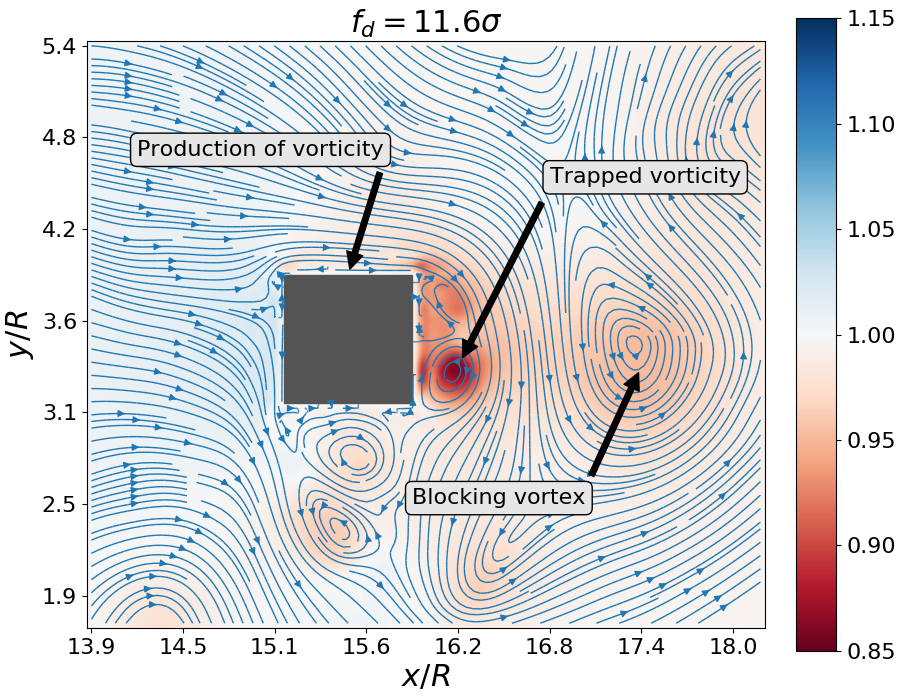
\includegraphics[width=.5\linewidth]{illustr_density_streamlines/illustr_density_streamlines.png}
\end{figure}

\begin{figure}
  \centering
  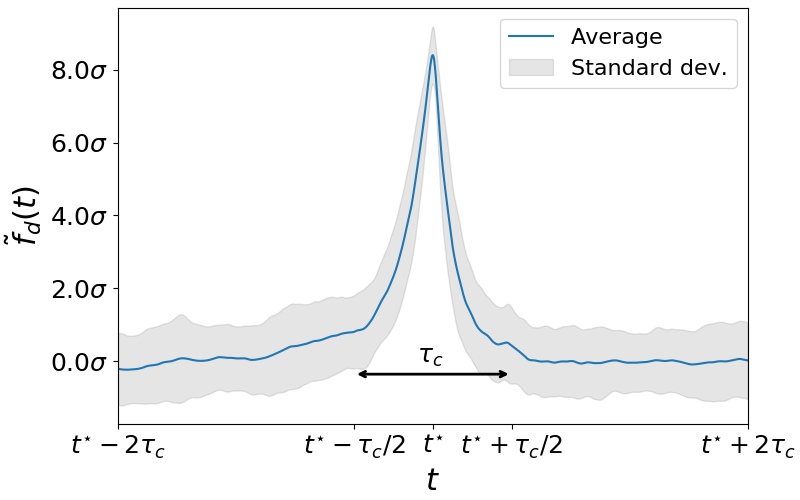
\includegraphics[width=.5\linewidth]{timeseries_extremes/timeseries_extremes.png}
\end{figure}

\begin{figure}
  \centering
  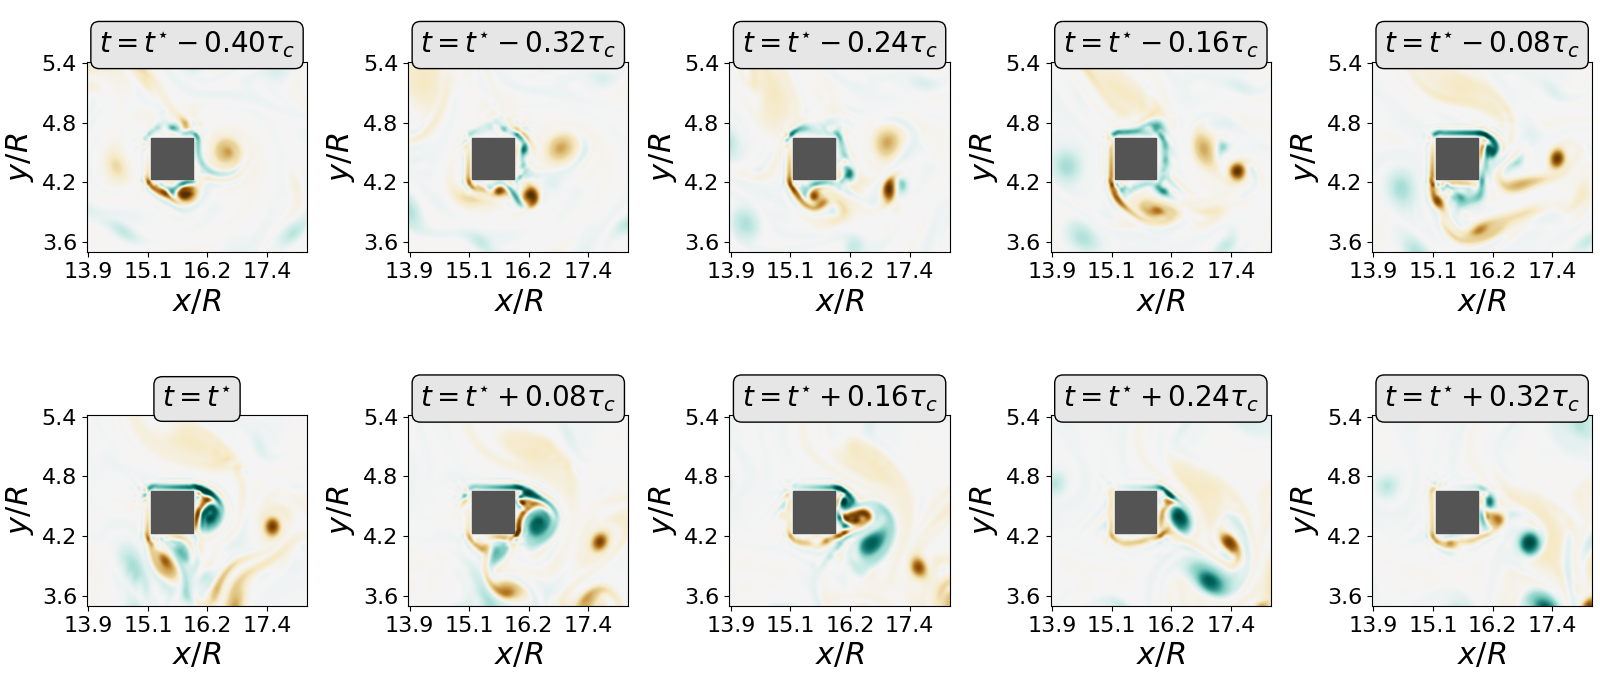
\includegraphics[width=.8\linewidth]{dynamics_extremes/dynamics_extremes.png}
\end{figure}

% \begin{figure}
%   \centering
%   \begin{minipage}{0.85\linewidth}
%     \begin{tabular}{c|c}
%     \subfloat[$f'_d = 11.6\sigma$]{\label{fig:top_4_events_vorticity_a}\includegraphics[width=0.4\linewidth]{event_95_vort.png}} \hspace{0.5cm} & \hspace{0.5cm} \subfloat[$f'_d = 11.2\sigma$]{\includegraphics[width=0.4\linewidth]{event_69_vort.png}} \\
%     \hline
%     \subfloat[$f'_d = 10.6\sigma$]{\includegraphics[width=0.4\linewidth]{event_53_vort.png}} \hspace{0.5cm} & \hspace{0.5cm} \subfloat[$10\sigma$]{\includegraphics[width=0.4\linewidth]{event_20_vort.png}}
%     \end{tabular}
%   \end{minipage}
% \begin{minipage}[h]{0.1\linewidth}
%   \centering
%   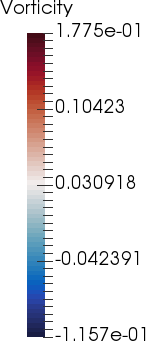
\includegraphics[width=\linewidth]{scale_vorticity.png}
% \end{minipage}
% \caption{\label{fig:top_4_events_vorticity} Vorticity field at $t=t^{\star}$ for the four highest drag fluctuations in the timeseries. The corresponding drag timeseries can be found in figure~\ref{fig:extremes_timeseries}.
%   The high value for the drag results from the formation of a strong negative (red) vortex inducing a pressure drop at the base of the obstacle. The formation of such a structure is aided by important vorticity production at the bottom boundary of the obstacle coupled with the influence of positive vorticity in the vicinity of the base.}
% \end{figure}  

% \begin{figure}
%   \centering
%   \begin{minipage}[h]{0.85\linewidth}
%     \begin{tabular}[h]{c|c}
%     \subfloat[$f'_d = 11.6\sigma$]{\label{fig:top_4_events_streamlines_a}\includegraphics[width=0.4\linewidth]{event_95_streamlines.png}} \hspace{0.5cm} & \hspace{0.5cm} \subfloat[$f'_d = 11.2\sigma$]{\includegraphics[width=0.4\linewidth]{event_69_streamlines.png}} \\
%     \hline
%     \subfloat[$f'_d = 10.6\sigma$]{\includegraphics[width=0.4\linewidth]{event_53_streamlines.png}} \hspace{0.5cm} & \hspace{0.5cm} \subfloat[$f'_d = 10\sigma$]{\includegraphics[width=0.4\linewidth]{event_20_streamlines.png}} 
%   \end{tabular}
% \end{minipage}
% \begin{minipage}[h]{0.1\linewidth}
%   \centering
%   \includegraphics[width=\linewidth]{scale_density.png}
% \end{minipage}
% \caption{\label{fig:top_4_events_streamlines} Density field at $t=t^{\star}$ for the four highest drag fluctuations in the control simulation for \tf{2}. Recall that the density $\rho$ is proportional to the pressure $p$, following the ideal gas state equation $p=c_s^2\rho$. See chapter~\ref{chap:test_flows} and appendix~\ref{app:lbm}. Additionally, velocity streamlines are depicted, representing advection by the flow at $t=t^{\star}$, see note~\ref{note:streamlines}. Blue areas indicate areas of lower pressure while red regions indicate regions of higher pressure. The formation of a vortex very close to the base boundary leads to a strong pressure drop. The downstream vortices originating from the top boundary layer separation are clearly visible and constrain the formation of the base vortex to a region very close to the base boundary.}
% \end{figure}

% \begin{figure}
%   \centering
%   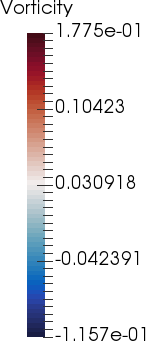
\includegraphics[width=0.1\linewidth]{scale_vorticity.png}
%   \begin{tabular}[h]{cccc}
%     \subfloat[$t = t^{\star}-0.54\tau_c$]{\label{frame_a}\includegraphics[width=.2\linewidth]{animation_event_95_0035}} & \subfloat[$t = t^{\star}-0.5\tau_c$]{\label{frame_b}\includegraphics[width=.2\linewidth]{animation_event_95_0036}} &     \subfloat[$t = t^{\star}-0.46\tau_c$]{\label{frame_c}\includegraphics[width=.2\linewidth]{animation_event_95_0037}} &     \subfloat[$t = t^{\star}-0.44\tau_c$]{\label{frame_d}\includegraphics[width=.2\linewidth]{animation_event_95_0038}} \\
%     \subfloat[$t = t^{\star}-0.4\tau_c$]{\label{frame_e}\includegraphics[width=.2\linewidth]{animation_event_95_0039}} &     \subfloat[$t = t^{\star}-0.36\tau_c$]{\label{frame_f}\includegraphics[width=.2\linewidth]{animation_event_95_0040}} &     \subfloat[$t = t^{\star}-0.34\tau_c$]{\label{frame_g}\includegraphics[width=.2\linewidth]{animation_event_95_0041}} &     \subfloat[$t = t^{\star}-0.3\tau_c$]{\label{frame_h}\includegraphics[width=.2\linewidth]{animation_event_95_0042}} \\
%     \subfloat[$t = t^{\star}-0.26\tau_c$]{\label{frame_i}\includegraphics[width=.2\linewidth]{animation_event_95_0043}} &     \subfloat[$t = t^{\star}-0.24\tau_c$]{\label{frame_j}\includegraphics[width=.2\linewidth]{animation_event_95_0044}} &     \subfloat[$t = t^{\star}-0.2\tau_c$]{\label{frame_k}\includegraphics[width=.2\linewidth]{animation_event_95_0045}} &     \subfloat[$t = t^{\star}-0.16\tau_c$]{\label{frame_l}\includegraphics[width=.2\linewidth]{animation_event_95_0046}} \\
%     \subfloat[$t = t^{\star}-0.12\tau_c$]{\label{frame_m}\includegraphics[width=.2\linewidth]{animation_event_95_0047}} &     \subfloat[$t = t^{\star}-0.08\tau_c$]{\label{frame_n}\includegraphics[width=.2\linewidth]{animation_event_95_0048}} &     \subfloat[$t = t^{\star}-0.04\tau_c$]{\label{frame_o}\includegraphics[width=.2\linewidth]{animation_event_95_0049}} &     \subfloat[$t = t^{\star}$]{\label{frame_p}\includegraphics[width=.2\linewidth]{animation_event_95_0050}} \\
%   \end{tabular}
%   \caption{\label{fig:type_1_event}Flow dynamics corresponding to a particular type 1 event, which drag timeseries and flow fields at $t=t^{\star}$ are displayed in figures~\ref{fig:extremes_timeseries}, \ref{fig:top_4_events_vorticity} and~\ref{fig:top_4_events_streamlines}, respectively. In each frame the vorticity field is displayed, as well as the velocity streamlines, representing advection by the flow at each instant. See note~\ref{note:streamlines} for a discussion of streamlines.
%     The maximum of the drag is attained for $t=t^{\star}$ and corresponds to frame~\ref{frame_p}.  The sequence starts with a shear boundary layer forming over the top boundary of the obstacle (frames~\ref{frame_a} to~\ref{frame_d}). This boundary layer separates (frames~\ref{frame_e} to~\ref{frame_j}) and results in the formation of a large positive eddy in the vicinity of the base of the obstacle (frames~\ref{frame_k} and~\ref{frame_l}). In the meantime, frames~\ref{frame_j} to~\ref{frame_m} depict the formation of an attached strong shear layer at the bottom boundary. Eventually, frames~\ref{frame_n} to~\ref{frame_p} illustrate that this results in vorticity production very close to the base, aided by the large positive eddy originating from the top boundary layer separation.}
% \end{figure}


We now turn to a description of the flow dynamics that correspond to extremely high values of the drag acting on the square obstacle.

Figure~\ref{fig:timeseries_extremes} displays the average of the drag timeseries corresponding to the 104 extreme events sampled in the control run, in the vicinity of the fluctuation.
It illustrates that extreme drag fluctuations are very local in time, with a lifetime of roughly one correlation time unit.
Starting from typical values, extreme drags are typically reached in less than a correlation time.
Moreover, such very high drag levels do not persist over time.
To understand why it is so, it is useful to visualize the corresponding flow fields.

To begin with, figure~\ref{fig:top_four_events} displays the vorticity field corresponding to the peak drag value, for a subset of the extreme events sampled in the control simulation.
We observe that, in each case, extreme drag flcutuations correspond to very similar flow configurations.
More precisely, a region of strong vorticity is located in the vicinity of the base of the obstacle, where vorticity levels typically reach twice as much as the typical vorticity fluctuations displayed in figure~\ref{fig:typical_event}.
This vorticity results from a boundary layer, along either the top or bottom side of the obstacle.
Such extreme vorticity is responsible for a significant pressure drop in the vicinity of the base of the obstacle, which in turn leads to an extreme value of the drag, see figure~\ref{fig:pressure_ratio}.

How are such vorticity reached ?
In contrast with the typical flow dynamics, illustrated in figure~\ref{vorticity_typical}, the vorticity generated within the boundary layers is not directly advectd by the means flow.
Figure~\ref{fig:illustr_density_streamlines} shows that, instead, this vorticity is constrained in the vicinity of the base of the obstacle.
Such constraint results from a large vortical region located roughly one obstacle length of the base, that prevents vorticity to be advected downstream.

Figure~\ref{fig:dynamics} illustrate the time evolution of the vorticity field, in the vicinity of the drag fluctuation, for the event depicted in figure~\ref{fig:illustr_density_streamlines}.
From $t^{\star}-0.4\tau_c$ to $t^{\star}-0.16\tau_c$, a strong negative eddy is generated along the bottom boundary layer of the obstacle and advected downstream by the mean flow.
This leads to a region of negative vorticity at roughly one obstacle length of the base of the obstacle, constraining the positive vorticity generated along the top boundary.
However, it can be seen in figure~\ref{fig:dynamics} that the positive vorticity only accumulates for a short duration.
The blocking negative vortex is in turn advected downstream, thus freeing the trapped positive vorticity.

The lifetime of an extreme drag fluctuation therefore corresponds to the duration over which the blocking vortex remains in the vicinity of the base.
Consistently with figure~\ref{fig:timeseries_extremes}, this duration is roughly one correlation time unit $\tau_c$.


We found that $80\%$ of the extreme events sampled from the control timeseries can be related to very similar dynamics.
In order to identify such events, we monitored the averaged shear along the top or bottom boundary
\begin{equation}
  \label{eq:avg_shear_def}
  \overline{\gamma} = \frac{1}{L} \int_{\mathcal{S}_b} \frac{\partial u_x(\mathbf{x})}{\partial y}\mathrm{d}\mathbf{x},
\end{equation}
where $L$ denotes the diameter of the cylinder, $u_x$ the longitudinal component of the velocity field and $\mathcal{S}_b$ the surface of either the top or the bottom boundary.
% Figure~\ref{fig:type_1_and_type_2_a} displays the label of the 104 sampled events, sorted according to the amplitude of the corresponding fluctuation.
% It illustrates that the dynamics corresponding to the large majority of events also corresponds to the events with the highest fluctuation amplitude.
Figure~\ref{fig:shear_asof_drag} shows $\overline{\gamma}$ as a function of the instantaneous drag $f_d$, for $t^{\star}-2\tau_c \leq t \leq  t^{\star}+2\tau_c$, for each of the sampled events that follow the previously described dynamics..
For $t^{\star}-2\tau_c \leq t \leq t^{\star}-\tau_c$ and $t^{\star}+\tau_c \leq t \leq t^{\star}+2\tau_c$, paths concentrate in the region describing typical values for both $\overline{\gamma}$ and $f_d$.
As illustrated in figure~\ref{fig:extremes_timeseries}, the drag abruptly varies for $t^{\star}-\tau_c \leq t \leq t^{\star}+\tau_c$.
As a consequence, paths in the $(f_d, \bar{\gamma})$ space display excursions to atypical values for both $\bar{\gamma}$ and $f_d$.
These excursions always go clockwise, that is, $\overline{\gamma}$ attains its maximum value before $f_d$ does.
This is consistent with an increase of $\overline{\gamma}$ acting as a precursor for extreme drag fluctuations.

The remaining $20\%$ of the sampled events correspond to slightly different dynamics.
In this case the vorticity responsible for the base pressure drop is not created along the top or bottom boundary, but directly through viscous shear alongside the base boundary of the obstacle.
This viscous shear is induced by a large vortex detached from the obstacle.
For a more detailed description of such dynamics, see the chapter 3 of ~\ref{ref:these_lestang}.

\begin{figure}
  \centering
  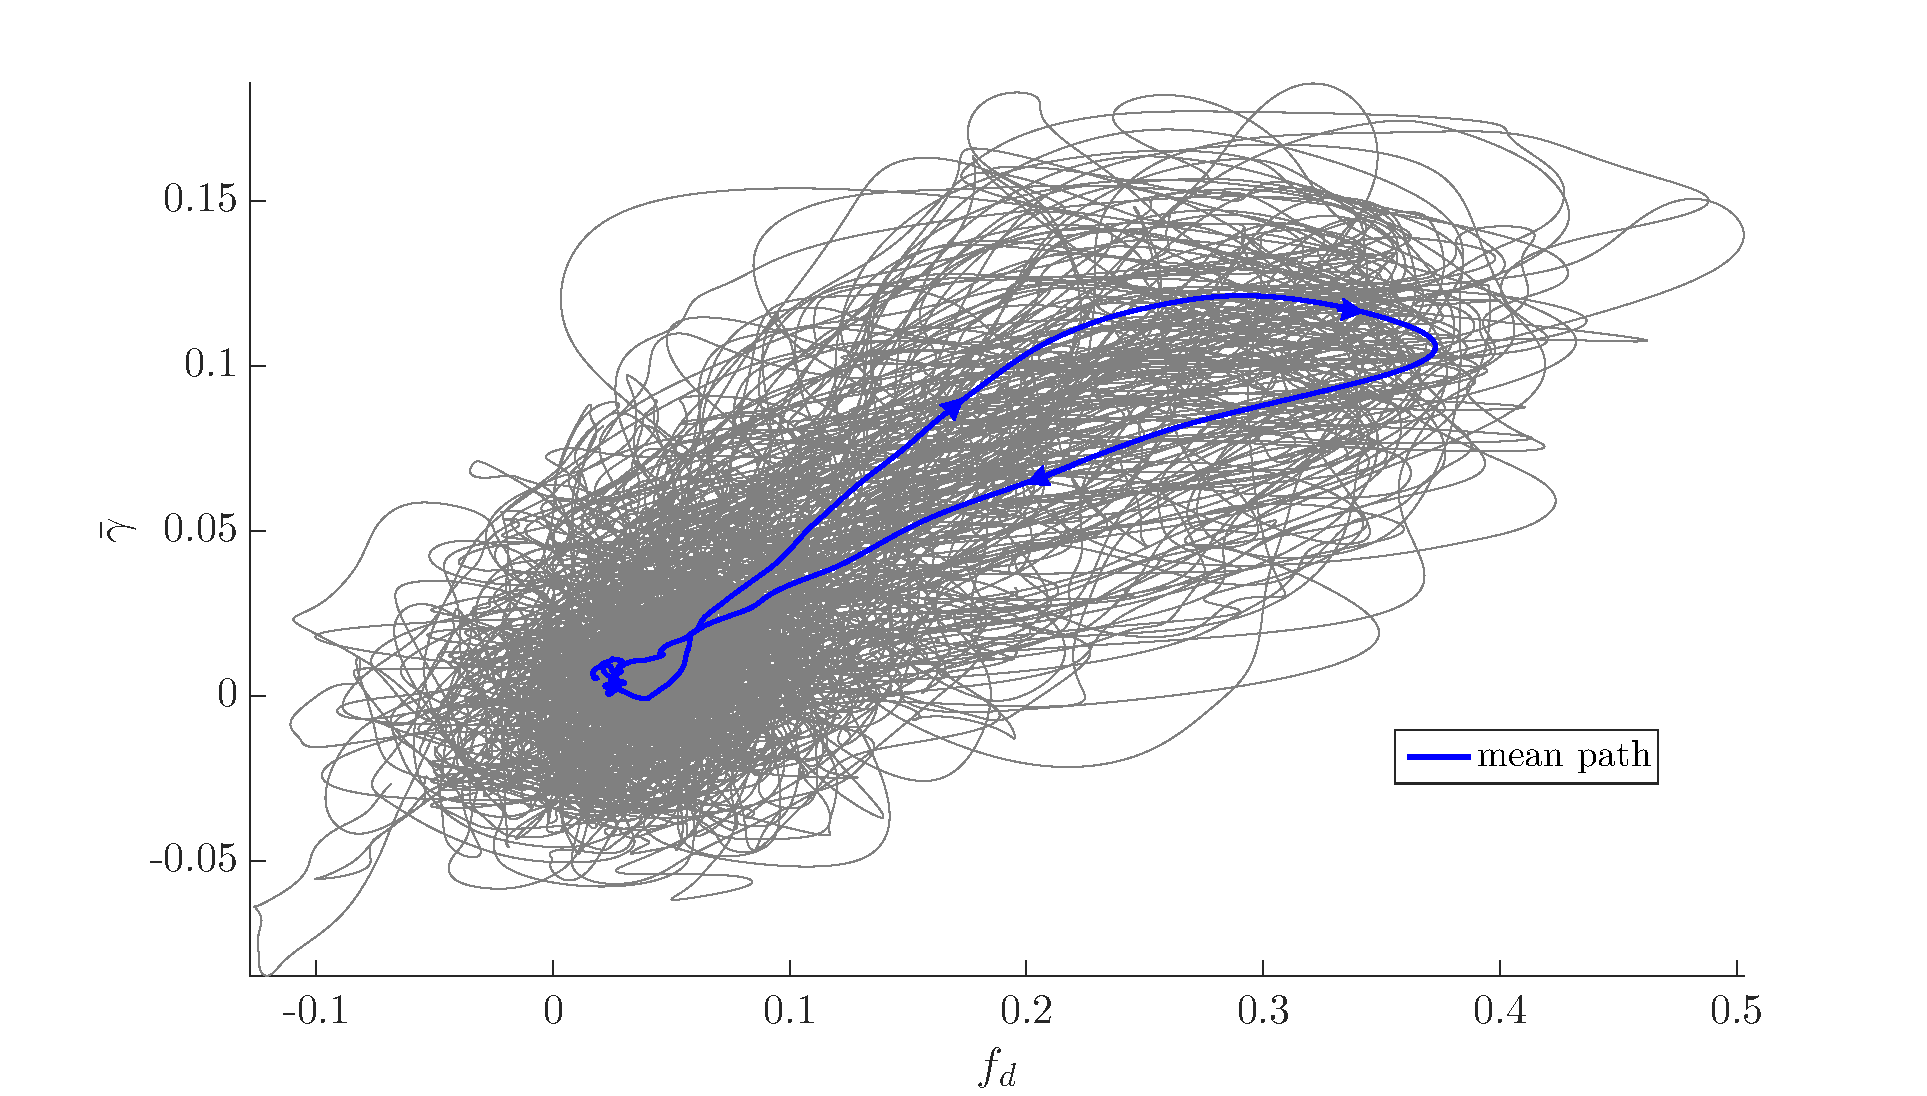
\includegraphics[width=.7\linewidth]{shear_asof_drag/shear_asof_drag}
  \caption{\label{fig:shear_asof_drag}}
\end{figure}

\subsection{Extreme fluctuations of the time-averaged drag }
\label{sec:time_avg}

% Motivation
In section~\ref{sec:instantaneous_drag}, we discussed the phenomenology of rare events corresponding to extremely high values of the drag acting on the square obstacle mounted in the flow described in section~\ref{sec:test_flow}.
In particular, it was pointed out that such extreme drag fluctuations have a lifetime of, roughly, one correlation time unit $tau_c$.
However, In many applications, this duration is much smaller than the timescale of interest.
Consider for insatnce the interaction of a deformable structure with a turbulent flow: the typical response time may be much larger than the lifetime of drag fluctuations.

%% Definition de la train�e int�gr�e
In such cases, a relevant observable is the \textit{time-averaged} drag
\begin{equation}
  \label{eq:def_time_averaged_drag}
  F_T(t) = \frac{1}{T}\int_t^{t+T} f_d(t) \mathrm{d}t,
\end{equation}
where $f_d$ denotes the instantaneous drag and $T\leq \tau_c$ a timescale of interest.
In the following we consider the case where $T \gg \tau_c$, typically $T=10\tau_c$.
In this context, a fluctuation of the average $F_T(t)$ is related to roughly $T / \tau_c$ independent fluctuations of the \textit{instantaneous} drag $f_d$, over the time interval $[t;t+T]$.

%% Quelle est la ph�nom�nologie de la train�e int�gr�e ?
What is the phenomenology leading to extreme values of $F_T(t)$ ?
Do an exceptionally large value of the average drag result from a single exceptionally large value of the instantaneous drag (case (1)) ?
Or instead from a succession of rather typical fluctuations, however all in the same direction (case (2)) ?
From the control timeseries, see section~\ref{sec:pdfs}, one can compute a control timeseries $\{F_T(t)\}_{0 \leq t \leq T_{tot}-T}$.
It is then possible to identify extreme positive fluctuations for which the time-averaged $F_T$ drag exceeds a fixed threshold $a$, in the very same way as described in section~\ref{sec:extreme_extraction}.
Setting $a=5.2\sigma _T$ leads to $84$ independent events, with $\sigma_T$ the standard deviation of the random process describing the time evolution of $F_T$.

Figure~\ref{fig:extreme_avg} displays the timeseries $\{f_d(t^{\star})\}_{t^{\star} \leq t \leq t^{\star}+T}$ for four of the sampled extreme fluctuations sampled in the control timeseries for $F_T$.
It illustrates that the phenomenology of the extreme fluctuations of the time-averaged drag can neither be reduced to case (1) nor case (2). 
Indeed, both cases are featured in figure~\ref{fig:extreme_avg}, along with intermediate cases where the very large value of the drag results from both a very large fluctuation and a large number of typical, however all positive, fluctuations of the instantaneous drag $f_d$.

This marginal phenomenology can be connected to the exponential shape of the tail of the \ac{pdf} describing extreme positive drag fluctuations~\cite{papier_JSTAT}.
An estimate of this \ac{pdf} is displayed in figure~\ref{fig:pdf_drag}.
Let $X$ be a random variable whose \ac{pdf} is denoted $\mathbb{P}$ and standard deviation $\sigma_X$.
Considering an extreme positive value $a$ of $S_N=\sum_{n=1}{N}X_n$, the probability $p_1$(resp. $p_2$) of case (1) (resp. case (2)) writes:   
\begin{equation}
  \label{eq:indep}
  p_{1}(\sum_{1}^{N} X_n=a) \approx \mathcal{P}\left(\frac{a}{N}\right)^{N} \,\,\, \text{and} \,\,\, p_{2}(\sum_{1}^{N} X_n=a)\approx \mathcal{P}(a)  
\end{equation}
If $\mathbb{P}$ has an exponential positive tail, \textit{i.e.} $\mathbb{P}(X=x) \underset{x \ll \sigma_X}{\propto} e^{-\alpha x}$, then both cases (1) and (2) are equiprobable, provided that the average $a=S_N/N$ is very large:
\begin{equation}
  \frac{p_{2}}{p_{1}} \underset{a\to \infty}{\sim} C\left(e^{-\alpha \frac{a}{N}}\right)^{N} e^{-\alpha a} = 1.
  \label{eq:ratio_exp}
\end{equation}

\section{Rare event algorithms}
\label{sec:rare_events_algorithms}

%% Limites de l'approche par �chantillonnage direct
In the limit of very rare events and/or very complex dynamics such as turbulent flows in industrial contexts, a direct sampling approach is unrealistic.
Indeed, according to equation~\eqref{eq:return_time_scaling}, the return time of a fluctuation $f_d \geq a$ verifies $r(a) \propto e^{\alpha a}$.
As a result, the computational cost required to sample events $f_d \geq a$ scales like $e^{\alpha a}$.

%% Objectif des algo.
In this section we discuss the application of \textbf{rare event algorithms} to the numerical sampling of extreme drag forces on immersed objects, on the example
of the flow presented in section~\ref{sec:test_flow}.
The purpose of rare events algorithms is to make it possible to sample rare events for a computational cost well inferior to their return time.
In sections~\ref{sec:ams} and~\ref{sec:gktl} we consider the \acl{ams} and \acl{gktl} algorithms, respectively.
Both algorithms rely on the simulation of an ensemble of $N$ trajectories $\{\mathbf{x}_n(t)\}_{1\leq n \leq N, 0\leq t T_a}$, where $\{\mathbf{x}(t)\}_{0\leq t T_a}$ is a formal notation for a trajectory
of duration $T_a$ in the phase space describing the dynamical system.
In this case the dynamical system is the flow described in section~\ref{sec:test_flow}.
Over the iterations of the algorithm, trajectories are duplicated or discarded from the ensemble according to precise selection rules that bias the sampling towards the rare events of interest.
Such selection rules are designed in such a way that the sampling bias is known at each iteration of the algorithm.
In other words, generated trajectories are given a statistical weight, which knowledge allows for the computation of both their probability and expectation values of any trajectory observables.

% In section~\ref{sec:ams}, we highlight that sampling  extreme fluctuations of the instantaneous drag with the \ac{ams} algorithm is a difficult task.
% In section~\ref{sec:gktl}, we apply an importance sampling algorithm, the \ac{gktl} algorithm, and efficiently sample rare trajectories corresponding to extreme fluctuations of the time-averaged drag.
% As an application, we use the \ac{gktl} algorithm to compute return times of very rare drag fluctuations.

\subsection{Extreme instantaneous drag forces with the \acl{ams} algorithm}
\label{sec:ams}
% Introduction to AMS
The \acl{ams}~\cite{amspaper} inherits from the basic ideas of \textit{splitting} algorithms~\cite{kahnharris}: the sampling of a rare event is made easier by splitting the corresponding dynamical path into a sequence of events that can be sampled with a higher probability~\cite{glasserman,rolland_simonnet}.
Even though a large body of variants have been proposed since the early 50s, the \ac{ams} appears as the most advanced formulation of multilevel splitting to date (\textbf{Sans doute un peu <<too-much>>. Avec cette phrase je voudrais justifier que l'on s'int�resse � l'AMS et pas � un autre algo.}).
In recent years, it was applied to several problems, for instance the computation of the dissociation time of biomolecules~\cite{teo2016} or the simulation of rare relaminarizations in a stochastic model of wall turbulence~\cite{rolland2017}.

% Quick description of TAMS
In the present paper we use a variant of the \ac{ams} algorithm called the \ac{tams}.
The \ac{tams} relies on the definition of a time-dependant \textit{score function} $\xi (\mathbf{x}(t),t)$, as well as an iterative procedure starting from an ensemble $\{\mathbf{x}_n(t)\}_{1\leq n \leq N, 0\leq t T_a}$ of independant trajectories.
Each iteration consists in discarding the trajectories with the lowest maxima of the score function $\xi$ over the whole trajectory of duration $[0;T_a]$.
Discarded trajectories are resampled based on member of the ensemble of trajectories that achieved a higher value of the score function at some point of their history.
As an illustration, a particular iteration of the \ac{tams} algorithm is sketched in figure~\ref{figure_AMS}.
For further details about the algorithm and corresponding mathematical results, see~\cite{lestang2018} and references therein.

% Example: OU process
We first describe results of the \ac{tams} on a simple case.
We temporarily let fluid dynamics aside and consider a one-dimensional \ac{ou} process
\begin{equation}
  \label{eq:ou}
  \dot{x} = -x + \sqrt{2\epsilon}\eta (t)  
\end{equation}
We apply the \ac{tams} to simulate trajectories $\{x(t)\}_{0\leq t \leq T_a}$ with $\underset{0\leq t \leq T_a}{\max} x(t) \geq a$ with $a$ very large with respect to typical fluctuations of $x(t)$.
For the sake of simplicity, a single trajectory is resampled at each iteration of the \ac{tams}.
We denote by $a_j$ the maximum of the resampled trajectory at iteration $j$.
The computational cost of the algorithm after iteration $j$ is the computational cost of simulating the $N$ initial trajectories, as well as the resampling of the $j$ trajectories.
Figure~\ref{fig:compraison_temps_de_retour} illustrates that the successice resamplings of the \ac{tams} algorithm leads to trajectories displaying extreme fluctuations $x \geq a$.
More importantly, these very rare trajectories are sampled for a computational cost that several order of magnitude lower than the return time of the corresponding fluctuations.

Undoubtedly, an \ac{ou} process is an oversimplified dynamics to showcase the efficiency of the \ac{ams} and \ac{tams}.
Indeed, the state space is one-dimensional and the choice of the score function poses no questions: it is simply the observable $x$ itself.
In addition, the noise term in~\eqref{eq:ou} has no correlations in time, which means that newly generated trajectories will quickly separate from their ancestors.

% Application to turbulent flow past an obstacle
Can the \ac{tams} achieve similar results when applied to complex chaotic dynamics, such as turbulent flows around objects ?
To answer this question, we consider again the two-dimensional test flow introduced in section~\ref{sec:test_flow}.
Our aim is to sample trajectories that display extreme fluctuations of the drag $f_d$ acting on the square obstacle.
However, by contrast with a simple \ac{ou} process, the phase space is higly-dimensional and the dynamics complex.
As a consequence the choice of the score function $xi (\mathbf{x}(t),t)$ is not so clear.
In the following we use the \ac{tams} with $\xi \equiv f_d$, which is the most simple choice for the score function.
For such complex dynamics however, there is no reasons for the drag itself to be a good measure of how far is a given state to regions of phase space where the drag is extreme.
Unfortunately, the choice of better score functions rely on a deep understanding of the physics of the rare events of interest, which is precisely what we are trying to achieve.

% Commentaire figure instant_256_20

We apply the \ac{tams} with $N=256$ initial trajectories, with a duration $T_a = 20 \tau_c$.
Similarly to figure~\ref{fig:comparaison_temps_de_retour}, figure~\ref{fig:instant_256_20} displays the maximum drag achieved by resampled trajectories.
Figure~\ref{fig:instant_256_20} also shows the distribution of the maximum achieved drag for the $N$ \textit{initial} trajectories.
Over the first iterations of the algorithm, trajectories with the lowest maximum of the score function are discarded, and new trajectories with higher maximum are resampled.
These maxima are depicted by the stars in figure~\ref{fig:instant_256_20}.
However, one can see that resampled trajectories never exceeds the amplitude of the highest maximum in the initial set of trajectories.

% Commentaire de la figure iter_181

Figure~\ref{fig:instant_256_20} can be better understood by visualising the drag signals corresponding to the last resampled trajectories.
Figure~\ref{fig:instant_256_20_b} displays the ensemble of trajectories after $181$ iterations of the \ac{tams} resampling procedure.
Comparison with figure~\ref{fig:instant_256_20_b} suggests that, utimately, trajectories are resampled from the same initial trajectory.
This phenomenon can be explained as follows.
Because the flow dynamics have a memory, it takes a certain time before a resampled trajectory separate from its parent.
In our case, this memory originates from the deterministic nature of the dynamics, which implies that two trajectories starting from infinitesimally close starting points will overlap over a timescale called
the <<Lyapunov timescale>>~\cite{lyapunovRef}.
However, we observe that, in our particular case, the duration of extreme drag fluctuations is typically 5 times smaller that the Lyapunov timescale of the drag process.
This means that the resampling of a trajectory based on the value of the drag at $t^{\star}$ cannot lead to larger drag values for $t^{\star} \leq t \leq \tau_L$.
For $t > \tau_L$, the drag process has no memory of the drag fluctuations on which the resampling was based.
As a consequence, the probability of observing an extreme fluctuation over $\tau_l \leq t \leq T_a$ is very low.
The difference between the typical duration of drag fluctuations $\tau_c$ and the Lyapunov timescale $\tau_0$ is linked to the convective nature of the flow.
As described in section~\ref{sec:instantaneous_drag}, extreme fluctuations of the instantaneous drag $f_d$ have a lifetime of roughly $\tau_c$.
Fluid structures responsible for a particular value of the drag on the obstacle at a time $t^{\star}$ are swept away by the mean flow over a timescale $\tau_c$, shorter than the time it takes for
trajectories to separate, \textit{i.e} the Lyapunov timescale. 

% perspectives
This result suggest that the \ac{tams}--- and \ac{ams}---cannot be expected to efficiently sample rare trajectories for dynamics with such a phenomenology.
% More trajectories ?
Note that, because of the complexity of the dynamics, we were limited to a rather low number of trajectories, relatively to previous use cases of these algorithms~\cite{refs}.
Targeting events with a fixed return time, one can show that the computational cost of a \ac{tams} experiment roughly grows linearly with the number of trajectories $N$~\cite{lestang2018}.
As a result, multiplying the number of trajectories by a factor 10 or 100 would require important computational resources as well as an efficient parallel implementation of the \ac{tams}.
Despite the relative simplicity of the \ac{tams} algorithm, the latter implementation is difficult to achieve~\cite{ref}.
In any cases, from the observations made in this section, we do not expect that increasing the number of trajectories is able to better the efficiency of the sampling for such dynamics.
% Another score function ?
%%
% The choice of the simple score function was already discusses above...
% Maybe not necessary to RE-discuss it here.

% Modify the TAMS to fit the phenomenology ?
A promising perspective is to adapt the \ac{tams} to dynamics for which the Lyapunov time is larger than the typical duration of extreme events, such as the convective flow involved in this work.
In the original \ac{tams}, at later stages of the algorithm, new trajectories are resampled starting from points very close to the maximum of the parent trajectory.
Resampled trajectories have no chance to display a significantly higher maximum as they overlap their parent trajectory over the Lyapunov timescale.
As an example, the resampling procedure could be modified so that new trajectories are resampled roughly a Lyapunov time \textit{before} the maximum is attained.
In this way, it gives the opportunity for new events, associated to a higher fluctuations, to occur.
However, such modification(s) of the resampling procedure must be implemented with care, so as to preserve the mathematical properties of the \ac{ams} and \ac{tams}.
\begin{figure}
  \centering
  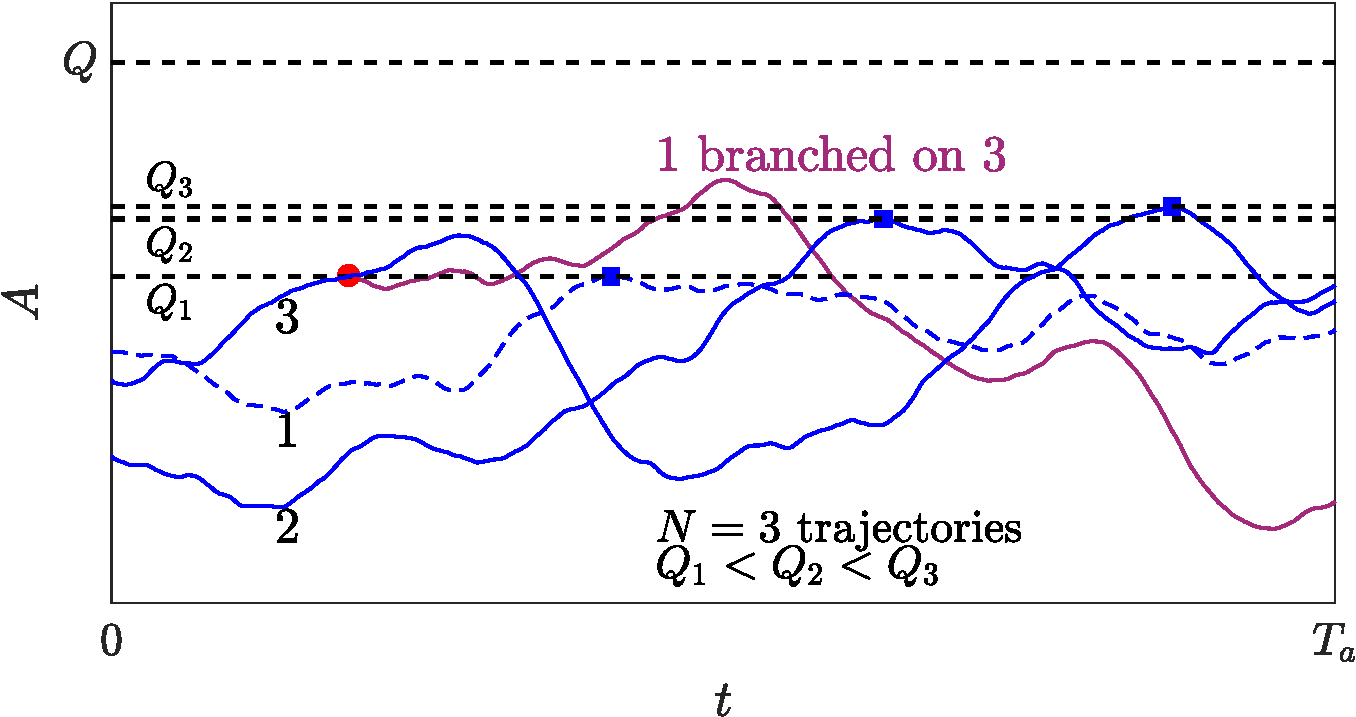
\includegraphics[width=.7\linewidth]{illustr_AMS/figure_AMS}
  \caption{Illustration of one selection-mutation step in the \ac{ams} algorithm for the computation of the probability that an observable $A:\mathbb{R}^d\to \mathbb{R}$  reaches values larger than $Q$ over a trajectory of duration $T_a$.}
\end{figure}
\begin{figure}
  \centering
  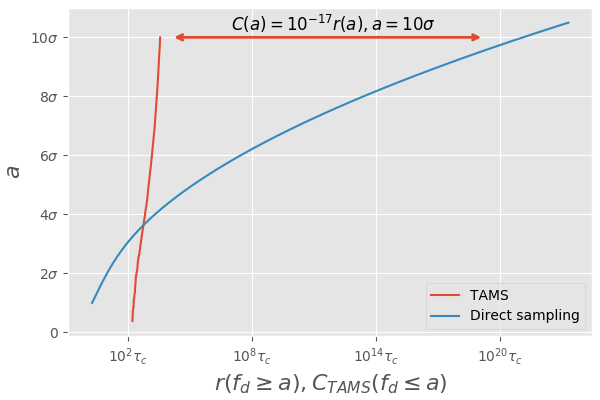
\includegraphics[width=.7\linewidth]{AMS_OU/AMS_OU.png}
    \caption{Illustration of the efficiency of the \ac{tams} algorithm with respect to direct sampling. The amplitude of fluctuations for the \ac{ou} process~\eqref{eq:OUprocess_chap_ams} are represented along the Y-axis. Along the X-axis is represented the typical computational cost required to sample fluctuations of the corresponding amplitude in both the \ac{tams} and direct sampling. In the latter, the typical computational cost is simply the return time $r(a)$. The computational cost associated to a level $a$ is the \ac{tams} is denoted by $C(a)$. The orange line represents the evolution of the level $\mathcal{Q}_j^{\star}$ as a function of the cost $C(a)$. The blue stars represent the maximum of $x(t)$ over the resampled trajectory \emph{after} it is resampled, that is at iteration $j+1$. Finally, the solid black line is the analytical solution for the return time of amplitude $a$~\cite{lestang_computing_2018}.}
  \label{fig:comparaison_temps_de_retour}
\end{figure}

\begin{figure}
  \centering
  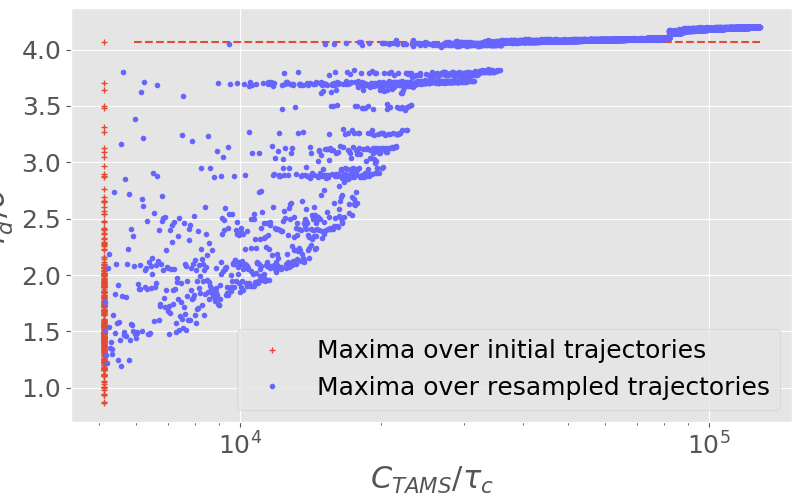
\includegraphics[width=.7\linewidth]{AMS_drag_resampling/AMS_drag_resampling.png}
    \caption{Maximum of the instantaneous drag along the resampled trajectories, denoted by $\tilde{f}_d^{(j)}$, as a function of the corresponding computational cost $C_j$, defined in~\eqref{eq:comp_cost_iterations}. In both figures, the \ac{tams} is iterated until extinction. 
    The solid black line indicates the typical fluctuation amplitude $a$ as a function of the corresponding  \textit{return time} $r(a)$. It is the typical timescale of occurrence of fluctuations above $a$. Furthermore, the square markers depict the maximum $\tilde{f}_{d,n}^{(0)},\,\, 1\leq n \leq N_c$ over the initial trajectories.
    This figure illustrates that in both experiments the \ac{tams} does not improve the sampling of rare fluctuations. On can see that the maximum values among the resampled trajectories concentrates on values already sampled over the initial trajectories. Eventually, extinction is reached as the algorithm is unable to generate a fluctuation higher than the maximum fluctuation in the initial ensemble of trajectories.
    This behaviour is illustrated in figure~\ref{fig:extinction_32_5} on the basis of the drag timeseries involved in the experiment of figure~\ref{fig:comparaison_ams_return_time_instant_a}.}
\end{figure}

\begin{figure}
  \centering
  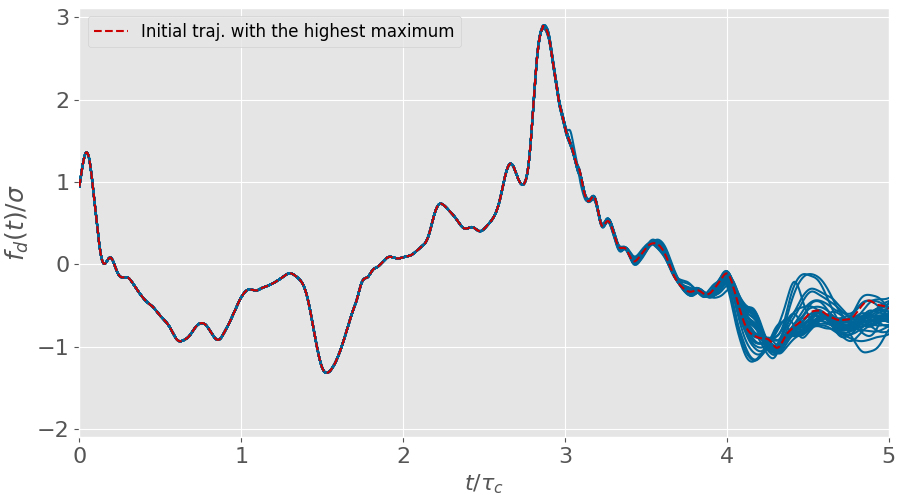
\includegraphics[width=.7\linewidth]{AMS_drag_trajectories/AMS_drag_trajectories.png}
    \caption{Visualisation of the drag timeseries corresponding to the set of trajectories in the ensemble, at different iterations along the algorithm. In this experiment, the \ac{tams} is used with the instantaneous drag $f_d$ as a score function. Trajectories have a duration $T_a = 5\tau_c$ and their number is $N_c = 32$.
    One can see that, as the number of iterations increases, the number of independent resampled trajectories drastically decreases until extinction at iteration $181$. The timeseries corresponding to the two initial trajectories exhibiting the highest fluctuations are displayed in colour. In all four figures, colour is inherited from the parent trajectory. It illustrates that the two strongest initial trajectories quickly become predominant in the ensemble, as the other are discarded.
    As can be seen in figure~\ref{fig:subfigc}, trajectories only separate well after the maximum is reached. Therefore, resampling the blue trajectories based on the red trajectories can only change the overall maximum by a very small amount. Consequently, blue trajectories are discarded one after the other, each time resampled into another instance of the red trajectory. This new instance has roughly the same maximum as the others.}
\end{figure}

\subsection{Extreme time-averaged drag forces with the \acl{gktl} algorithm}
\label{sec:gktl}

We now turn to the sampling of extreme fluctuations of the time-averaged drag $F_T$.
The \ac{tams} algorithm could be used in the same way as described in section~\ref{sec:ams} for the instantaneous drag, choosing $F_T$ itself as a score function.
However, this leads to the same problem: the resampling fails to efficiently generate new, higher fluctuations of $F_T$.

For time-averaged observables, one can make use of a different algorithm: the \acf{gktl} algorithm~\cite{Giardina2006,Tailleur2007,Giardina2011}.
It was originally designed to compute large deviations rate functions of time-averaged dynamical observables, that describe the probability density of both typical of rare events in the limit of large
averaging time~\cite{ref_large_dev}.
By contrast with the \ac{ams} and \ac{tams}, the \ac{gktl} algorithm does not follow the strategy of splitting algorithms.
Instead, it implements \textit{importance sampling}, \textit{i.e.} sampling a modified distribution that is biased towards the rare events of interest.
The idea of importance sampling is very general and was used in many different contexts (see e.g.~\cite{Berg1992,Hartmann2002} and the general references~\cite{Bucklew2004,RubinoTuffin2009}). 
The \ac{gktl} algorithm performs importance sampling in the space of trajectories, which is relevant for out-of-equilibrium systems.

\subsubsection{The \ac{gktl} algorithm}
\label{sec:gktl_description}
Similarly to the \ac{tams} algorithm, the \ac{gktl} relies on the simulation of a ensemble of trajectories.
In this case however, they interact dynamically: at regular time intervals, some members of the ensemble are killed and some are cloned according to a weight which depends on the history of the replica.
The weights are chosen such that, after several iterations of the algorithm, generated trajectories are distributed according to a probability distribution that is biased in favour of trajectories with large values of the time-averaged observable of interest.
The \ac{gktl} algorithm belong to a family of algorithms known as <<Go with the winners>>~\cite{aldous_varizani,grassberger}.
Similar ideas have been applied in a wide range of fields over the past 50 years, under different names, depending of the specific application domain~\cite{delMoral_Feynman_Kac_book}.
The application of a Go with the winners approach to the computation of large deviations in non-equilibrium systems has first been proposed in 2006~\cite{Giardina2006}.
Over the past ten years, it has successfully been applied to investigate rare events in both stochastic~\cite{Giardina2006,Lecomte2007b,Garrahan2007,Hurtado2009b} and deterministic systems~\cite{Giardina2006,Tailleur2007}.

The \ac{gktl} algorithm consists in simulation an ensemble of $N$ trajectories $\left\{\mathbf{x}_{n}(t)\right\}_{1 \leq n \leq N}$ starting from independant random initial conditions.
Similarly to section~\ref{sec:ams}, the total integration time of the trajectories is denoted $T_{a}$.
We consider an observable of interest $A(\mathbf{x}(t))$ and a cloning period $\tau$.
At times $t_{i}=i\tau$ (with $i=1,2,...,T_{a}/\tau$) we assign to each trajectory $n$ a weight $W_{n}^{i}$ defined as
\begin{equation}
W_{n}^{i}=\frac{e^{k\intop_{t_{i-1}}^{t_{i}}A(X_{n}(t))dt}}{R_{i}}\,\,\,\mbox{with}\,\,\,R_{i}=\frac{1}{N}\sum_{n=1}^{N}e^{k\int_{t_{i-1}}^{t_{i}}A(X_{n}(t))dt}.\label{eq:Weight}.
\end{equation}
For each trajectory $\{\mathbf{x}_{n}\}_{0 \leq t_i}$, a random number of copies of the trajectory are generated.
This number is on average proportional to the weight $W_{n}^{i}$, such that the total number of trajectories produced at each event is equal to $N$.
For deterministic systems, a small perturbation is introduced for clones at times $t_i$, so that clones separate from their parent. 
The parameter  is chosen by the user in order to control the strength of the selection.
The free parameter $k$ sets the amplitude of the typical fluctuations within the biased ensemble of trajectory sampled by the algorithm.
A higher value of $k$ will give a higher weight to higher fluctuations, thus driving the sampling to more extreme events.

Let us denote formally $\mathbb{P}_{0}\left(\left\{ X(t)\right\} _{0\leq t\leq T_{a}} = \left\{ x(t)\right\} _{0\leq t\leq T_{a}}\right)$ the probability to observe a trajectory $\left\{ x(t)\right\} _{0\leq t\leq T_{a}}$ in the model, and $\mathbb{P}_{k}\left(\left\{ X(t)\right\} _{0\leq t\leq T_{a}} = \left\{ x(t)\right\} _{0\leq t\leq T_{a}} \right)$ the probability to observe the same trajectory with the algorithm.
By construction of the algorithm through the weights~\eqref{eq:Weight}, we have
\begin{align}
\mathbb{P}_{k}\left(\left\{ X(t)\right\} _{0\leq t\leq T_{a}}=\left\{ x(t)\right\} _{0\leq t\leq T_{a}}\right) &\underset{N\rightarrow\infty}{\sim} \frac{e^{k\int_{0}^{T_{a}}A(x(t))dt}}{Z(k,T_a)}\mathbb{\mathbb{P}}_{0}\left(\left\{ X(t)\right\} _{0\leq t\leq T_{a}}=\left\{ x(t)\right\} _{0\leq t\leq T_{a}}\right).\label{eq:Biased_Path_Approximation}
\end{align}
where the normalisation factor is given by $Z(k,T_a)=\mathbb{E}_{0}\left[e^{k\int_{0}^{T_{a}}A(X(t))dt}\right]$, denoting by $\mathbb{E}_{0}$ the expectation value with respect to $\mathbb{P}_{0}$, and $\underset{N\rightarrow\infty}{\sim}$ means that this is true only asymptotically for large $N$.
The typical error is of order $1/\sqrt{N}$ when evaluating averages over observables.
Equation~\eqref{eq:Biased_Path_Approximation} is obtained by assuming the mean field approximation
\begin{equation}
R_{1}=\frac{1}{N}\sum_{n=1}^{N}e^{k\int_{0}^{t_{_{1}}}A(X_{n}(t))dt}\underset{N\rightarrow\infty}{\sim} Z(k,t_1)= \mathbb{E}_{0}\left[e^{k\int_{0}^{t_{1}}A(X(t))dt}\right],\label{eq:Mean_Field_Approximation}
\end{equation}
which, by induction, and using a formula similar to~\eqref{eq:Mean_Field_Approximation} at each step of the induction, leads to~\cite{Giardina2006,Giardina2011}:
\begin{equation}
\prod_{i=1}^{T_{a}/\tau}R_{i}\underset{N\rightarrow\infty}{\sim} Z(k,T_a) =\mathbb{E}_{0}\left[e^{k\int_{0}^{T_a}A(X(t))dt}\right].\label{eq:Estimate_Lambda}
\end{equation}
The validity of the mean field approximation and the fact that the typical relative error due to this approximation is of order $1/\sqrt{N}$ has been proven~\cite{DelMoralBook,DelMoral2013} to be true for a family of rare event algorithms including the one adopted in this paper.

Formula~\eqref{eq:Biased_Path_Approximation} is valid only for times $T_{a}$ that are integer multiples of the resampling time $\tau$.
The killed trajectories have to be discarded from the statistics.
Starting from the final $N$ trajectories at time $T_{a}$, one goes backwards in time through the selection events attaching to each piece of trajectory its ancestor.
In this way one obtains an effective ensemble of $N$ trajectories from time 0 to time $T_{a}$, distributed according to $\mathbb{P}_{k}$.
All trajectories reconstructed in this way are real solutions of the model: we have not modified the dynamics, but only sampled trajectories according to the distribution $\mathbb{P}_{k}$ rather than according to the distribution $\mathbb{P}_{0}$.

The sampled trajectories can be used to compute the statistical properties of any observable with respect to the distribution $\mathbb{P}_{0}$, from the distribution $\mathbb{P}_{k}$.
This is done using the backward reconstructed trajectories and inverting formula~\eqref{eq:Biased_Path_Approximation}.
For more details concerning the implementation of the algorithm and the corresponding data analysis, see~\ref{these_lestang,nemoto_bouchet2016}
As an example, say one wants to estimate the expectation value of an observable $O\left(\left\{ X(t)\right\} _{0\leq t\leq T_{a}}\right)$.
An estimator is then given by
\begin{equation}
\mathbb{E}_{0}\left[O\left(\left\{ X(t)\right\} _{0\leq t\leq T_{a}}\right)\right]\underset{N\rightarrow\infty}{\sim}\frac{1}{N}\sum_{n=1}^{N}O\left(\left\{ X_{n}(t)\right\} _{0\leq t\leq T_{a}}\right)\mbox{e}^{-k\int_{0}^{T_{a}}A(X_{n}(t))dt}\mbox{e}^{T_{a}\lambda(k,T_{a})},\label{eq:GK_O_estimator}
\end{equation}
where the $X_{n}$ are the $N$ backward reconstructed trajectories.
Events that can be considered rare with respect to $\mathbb{\mathbb{P}}_{0}$ are oversampled following $\mathbb{P}_{k}$.
As a result, the effective ensemble of trajectories generated by the \ac{gktl} algorithm contains a larger amount of such events, and empirical estimators such as~\eqref{eq:GK_O_estimator} have a dramatically lower statistical error.

\subsubsection{Application to extreme fluctuations of the time-averaged drag}
\label{sec:gktl_drag}

We now discuss the application of the \ac{gktl} algorithm to the flow dynamics introduced in section~\ref{sec:test_flow}.
The objective is to sample trajectories displaying extreme fluctuations of the \textit{time-averaged} drag~\eqref{eq:def_time_averaged_drag}.
Consistently with section~\ref{sec:time_avg}, we choose the averaging window $T=10\tau_c$.

% Choice of parameters and perturbation
The computational cost $C_{gktl}$ of a \ac{gktl} experiment is determined by both the duration of the trajectories $T_a$ and the number of trajectories $N_c$: $C_{gktl} = N_c \times T_a$.
In the following series of experiments we set $T_a = T = 10\tau_c$.
The sampling from the \ac{gktl} algorithm will be compared to the sampling from the control run, \textit{i.e.} a direct simulation of the flow over $T_{tot}=10^6\tau_c$.
We set $N_c=16384$, leading to $C_{gktl} \approx 1.6 \times 10^5 \tau_c$. (\textbf{Plus vraiment clair pour moi pourquoi je n'ai pas utilis� 10X plus de clones, pour matcher le co�t num�rique de la simulation de contr�le...})
Lastly, one must set the cloning period $\tau$.
On the one hand, too small a cloning period may result in loss of information: clones do not separate from their parent over a cloning period.
On the other hand, choosing $\tau \gg \tau_c$ may result in too few cloning stages to achieve importance sampling.
A rule of thumb is to set $\tau \approx \tau_c$.
In the following, we set $\tau = \tau_c /2$.

% Commentaire de la figure illustration_IS

We performed three experiments, corresponding to three different values of the parameter $k$.
In general the value of $k$ must be set empirically, unless a \textit{large deviation regime} $T_a \to \infty$ is verified~\cite{ref_ld_regime}.
In the latter case, the parameter $k$ can be related to the typical amplitude of the sampled fluctuations through the Gartner-Ellis theorem~\cite{GEref}.
% In the large time limit $T_a\to \infty$, the typical level of fluctuations $\mathbb{E}_{\mathbb{P}_k}[ F_{T_a} ]$ within the biased ensemble of trajectories
% can be related to the \textit{Scaled Cumulant Generating Function} $\lambda(k)$~\cite{ref}.

Figure~\ref{fig:illustration_IS} illustrates importance sampling achieved by means of the \ac{gktl} algorithm for the time-averaged drag $F_T$ with $T = T_a = 10\tau_c$.
For each of the three experiments, it displays the estimate of the biased \ac{pdf}
\begin{equation}
  \label{eq:estimate_biased_measure}
  \rho_k(F) = \mathbb{E}_{\set{P}_k}[\delta(F_{T_a}[\{\mathbf{x}\}_{0\leq t \leq T_a}]-F)]
  \approx \frac{1}{N_c}\sum_{j=1}^{N_c}\delta(F^{(j)}_{T_{a}}[\{\mathbf{x}\}_{0\leq t \leq T_a}] - F),
\end{equation}
computed over the set of $N=16384$ trajectories sampled by the algorithm.
Moreover, figure~\ref{fig:illustration_IS_drag} displays an estimate of the <<unbiased>> \ac{pdf} $\set{P}_0$ describing the time-averaged drag process.
Note that it corresponds to equation~\eqref{eq:estimate_biased_measure} with $k=0$.

% Limitations

For a fixed number of trajectories $N$, there is a limited range of $k$ values for which the algorithm is able to yield an accurate estimate of $\rho_k$.
Setting $k$ to too high a value causes harmful effects resulting from the finiteness of the ensemble of trajectories: trajectories overlap over most of their duration.
This effect is illustrated in figure~\ref{fig:illustration_IS}, where the histogram corresponding to the largest value of $k$ is peaked around a single value.
This is a consequence of the fact that most of the trajectories in the biased ensemble overlap, therefore leading to the same value for the averaged drag $F_T$.
See~\cite{ref1,ref2,ref3} for further details about the scaling of the required population size as $k$ is increased.

% Malgr� les limitations, c'est toujours mieux
% qu'un �chantillonnage direct
Unsurprisingly, sampling larger fluctuations requires a larger population size, and therefore a larger computational cost.
Even though, table~\ref{tbl:nbTraj_tbl} shows that the \ac{gktl} algorithm is able to sample trajectories corresponding to values of the time-averaged drag that could
not be sampled through a direct sampling with equal computational cost.
Table~\ref{tbl:nbTraj_tbl} displays the number of trajectories that correspond to a time-average $F_{T_a} \geq a$, for several values of $a$.
As a comparison, it also displays the average number of such fluctuations in a control timeseries of duration $C_{gktl}$, divided in $N_c = C_{gktl} / T_a$ events.
This number is computed based on the assumption that the \ac{pdf} describing the random variable $F_T$ with $T=10\tau_c$ is Gaussian.
This hypothesis is motivated by figure~\ref{fig:PDF_AVG}.
While this assumption does not hold for $F_T \geq 4\sigma_T$, it may still provide numbers relevant to the comparison with the algorithm.
\begin{figure}
  \centering
  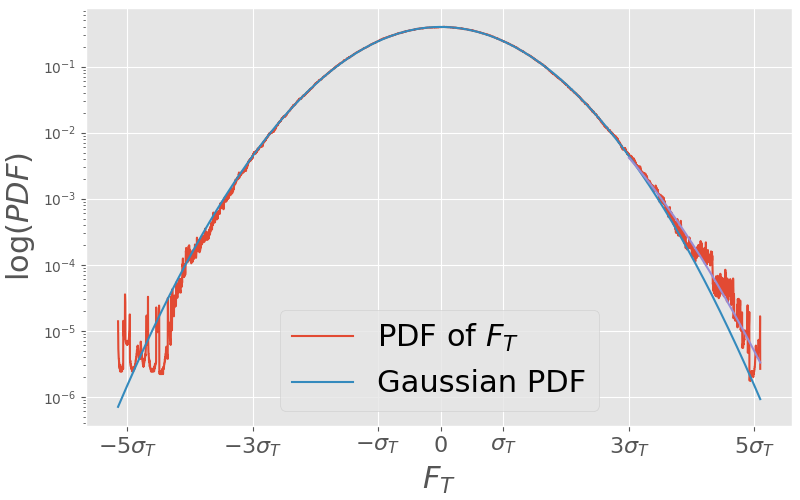
\includegraphics[width=.7\linewidth]{PDF_AVG/PDF_AVG}
  \caption{PDF of average drag over $10\tau_c$}
  \label{fig:PDF_AVG}
\end{figure}

In section~\ref{sec:time_avg} we observed that extremely large values of the time-averaged drag can either result from a succession of rather typical---however all positive---fluctuations of the instantaneous drag $f_d$, or from a small number of extremely large fluctuations of the instantaneous drag.
In the latter case, each fluctuation typically lasts a correlation time $\tau_c$.
In this context, the \ac{gktl} algorithm is particularly suited to sample trajectories that display a succession of these fluctuations.
(\textbf{conclusion � d�velopper.})
\begin{table}
  \centering
  \begin{tabular}{l|ccccc}
     & $\sigma$ & $2\sigma$ & $3\sigma$ & $4\sigma$ & $5\sigma$ \\
    \hline
    $k=0.02$ & 1594 & 799 & 155 & 22 & 0  \\ 
    $k=0.025$ 1019 & 834 & 521 & 198 & 27  \\ 
    $k=0.03$ & 539 & 510 & 391 & 205 & 36  \\ 
    $\mathcal{N}_{direct}$ & 2599.408 & 372.738 & 22.117 & 0.519 & 0.005  \\ 
  \end{tabular}
  \caption{Number of independent corresponding to fluctuations $F_{T_a} \geq a$ with a=$\sigma,2\sigma...$ in the biased ensemble, for the three experiments $k=0.02,0.025,0.03$. Parameters of the \ac{gktl} experiments are $N_c = 16384$, $T_a=10\tau_c$, $\tau = \tau_c /2$. Within the biased ensemble, trajectories are considered distinct if they overlap for less than $50\%$ of their duration.
    In addition, $\mathcal{N}_{direct}$ is the average number of fluctuations $F'_{T_a} \geq a$ on can expect from $N_c$ independent realisations of $F_{T_a}$, \textit{i.e.} with $k=0$.
    This number is based on the fact that the \ac{pdf} of $F_{T_a}$ is Gaussian.}
\label{tbl:nbTraj_tbl}
\end{table}

\begin{figure}
  \centering
%  \includegraphics[width=0.7\linewidth]{illustration_IS}
  \caption{\textbf{(a)}: Importance sampling for the time-averaged drag acting on the obstacle embedded in the test flow. The drag is averaged over $T=10\tau_c$. 
  The \ac{gktl} algorithm is used with $N_c = 16384$ copies and $T_a = T= 10\tau_c$ for three increasing values of the bias $k$. Additionally, the cloning period is $\tau = \tau_c/2$, resulting in $M=20$ iterations of the evolution/selection procedure. Note that in this particular example the last cloning stage at $t_{19}$ is not performed.
  As $k$ is increased, the sampled \ac{pdf} is shifted towards extreme values.
  Along the X-axis we display the fluctuation $F'_{T} = F_{T} - \overline{F_{T}}$, where the average $\overline{F_{T}}$ and standard deviation $\sigma_{T}$ have been computed over a timeseries spanning $10^6\tau_c$.
  One can see that the distribution for $k=0.03$ is peaked for a particular value of the fluctuation. This indicates that a significant part of the sampled trajectories actually overlap over the major part if their history.
  A a result, the average drag only differ by a small amount.}
\end{figure}

\section{Conclusion}
\label{conlusion}


\end{document}
%%% Local Variables:
%%% mode: latex
%%% TeX-master: t
%%% End:
